\documentclass[dvipsnames]{article}
\usepackage[margin=0.8in,letterpaper]{geometry}
\usepackage{graphicx}
\usepackage{amsmath,amssymb}
\usepackage{authblk}
\usepackage[T1]{fontenc}
\usepackage{gentium}
\usepackage{newtxmath}
\usepackage{natbib}
\usepackage[final]{hyperref}
\usepackage{tikz}
\usepackage{xcolor}
\usepackage{fancyhdr}
\usepackage{siunitx}
\usepackage{titlesec}
\usepackage{multicol,setspace,booktabs}
\usepackage[nameinlink]{cleveref}
\usepackage{threeparttable}
\usepackage{adjustbox}
\usepackage{subfigure}
%\usepackage{junpan}
\usepackage[font=small]{caption}
\usepackage{multirow}
\usepackage{hang}

\setcounter{secnumdepth}{4}

% A schematic for data processing might be helpful
\usetikzlibrary{shapes,arrows}
\tikzset{font=\footnotesize}
\newcommand{\sg}[1]{{\color{MidnightBlue}{{[SG: \bf #1]}}}}
\newcommand{\dl}[1]{{\color{Plum}{{[DL: \bf #1]}}}}
\newcommand{\cl}[1]{{\color{WildStrawberry}{{[CL: \bf #1]}}}}
\newcommand{\ks}[1]{{\color{ForestGreen}{{[KS: \bf #1]}}}}

\newcommand{\ExternalLink}{%
    \tikz[x=1.2ex, y=1.2ex, baseline=-0.05ex]{% 
        \begin{scope}[x=1ex, y=1ex]
            \clip (-0.1,-0.1) 
                --++ (-0, 1.2) 
                --++ (0.6, 0) 
                --++ (0, -0.6) 
                --++ (0.6, 0) 
                --++ (0, -1);
            \path[draw, 
                line width = 0.5, 
                rounded corners=0.5] 
                (0,0) rectangle (1,1);
        \end{scope}
        \path[draw, line width = 0.5] (0.5, 0.5) 
            -- (1, 1);
        \path[draw, line width = 0.5] (0.6, 1) 
            -- (1, 1) -- (1, 0.6);
            }
    }

\pagestyle{fancy}
\fancyhf{}
\rhead{Boston Regional Datathon Spring 2021}
\lhead{S. B. Green, D. Li, C. Liu, and K. Sangani}
\cfoot{\thepage}

\hypersetup{
	colorlinks=true,       % false: boxed links; true: colored links
	linkcolor=Orchid,        % color of internal links
	citecolor=Orchid,        % color of links to bibliography
	filecolor=Orchid,     % color of file links
	urlcolor=Orchid         
}

\onehalfspacing

\renewcommand\Affilfont{\itshape\small}

\title{%

\includegraphics[width=0.5\textwidth]{data-open-logo.jpg}~
\\[1cm]
Boston Regional Datathon Spring 2021 \\
\vspace{0.5em}
\textbf{Lock Me If You Can: \\
Lockdown Adherence, Fatigue, and Effectiveness} \\[0.5em]
\large Team 6} 
\author[1]{Sheridan B. Green}
\author[1]{Daming Li}
\author[2]{Canyao Liu}
\author[3]{Kunal Sangani}
\affil[1]{Department of Physics, Yale University}
\affil[2]{Yale School of Management}
\affil[3]{Harvard Business School}

\date{March 7, 2021}

\graphicspath{{figures/}}

\begin{document}

\maketitle

\section{Topic question}

State governments in the United States and governments of countries across the world implemented different containment policies in an effort to reduce the spread of COVID-19. In practice, the outcomes of these measures can drift significantly from the stated policies due to enforcement, adherence, ``stay-at-home fatigue,'' and the policy content. These factors suggest a gap between policy ``by the letter'' and the true impact of its implementation. In this study, we address the following questions:

%
\begin{enumerate}
    \item How can we measure the true influence of lockdown policies, specifically in terms of changes in social distancing behavior?
    \item Does social distancing impact disease transmission? If so, how effective is government policy at changing social distancing behavior? 
    %How to understand the interplay between the spread of the disease, government's policies, and people's social distancing practices?
    %What determines differences in (1) containment policy measures and (2) actual social distancing behavior across states? \dl{here questions are meant to be broad so we don't have to give examples, and three questions are already a lot} \ks{Yeah - maybe we cut this last one?} \dl{yea, let's remove the last one}
    %For example, does political affiliation affect the severity of lockdown and/or adherence to the stated policies? 
    %\item How voters of different parties (Democratic versus Republican) behave in terms of social distancing and how does that explain the difference in virus spread for different states?
\end{enumerate}
%

Our answers to these questions provide crucial insights towards understanding patterns of disease spread and evaluating the effectiveness of public health policies.
\pagebreak
\section{Executive summary}
One question that has dominated discourse during the COVID-19 pandemic is how government lockdowns can mitigate disease spread. In response, popular datasets, such as the Oxford Coronavirus Government Response Tracker (OxCGRT), have tracked lockdown severity by recording and scoring government lockdown policies.\footnote{The OxCGRT tracker was provided to us on a country-level as part of the Data Open datathon materials; in our study, we supplement this data with records at the state level provided directly from OxCGRT. These indicators have been widely cited as a measure of containment. See, for example, the \href{https://www.nytimes.com/interactive/2020/11/18/us/covid-state-restrictions.html}{New York Times \ExternalLink} and \href{https://www.wsj.com/articles/measuring-the-strictness-of-your-lockdown-a-university-boils-it-down-to-one-number-11590246001}{Wall Street Journal \ExternalLink}.} In practice, however, the true level of social distancing may deviate from regional laws due to (1) enforcement and (2) adherence (which is in turn affected by social norms, lockdown fatigue, and business practices). As a result, measuring disease containment using policy ``by the letter'' may miss important components of the true incidence of a lockdown as reflected by the change in human behavior.
%misses an important component of 

To this end, we create a shadow measure of lockdown severity, which we refer to as the \textbf{Social Distancing Index (SDI)}. Our index incorporates a wide array of regional data made available during the pandemic, such as seatings at local restaurants, GPS-based mobility data, and small business openings and revenues. We use dimensionality reduction techniques to isolate the dominant component of these data, thereby creating a shadow indicator on the severity of lockdown, available on a daily basis, that reflects the degree to which a population is practicing reduced mobility and contact.

%We begin by plotting the time courses of daily death increase, containment index, and the SDI to visualize the interplay between the severity of the pandemic, government policy, and people's actions. Near mid-March 2020, we observe a surge in each one of these variables, which marks the beginning of the pandemic. The death numbers dropped in the summer and then dramatically increased back in winter. On the other hand, the containment index remained relatively stable near its peak value since the summer, whereas SDI dropped in summer and has remained flat since then despite the second wave of the disease. We also observe strong heterogeneity across states. These interesting temporal patterns motivate us to further analyze their relationships. \ks{This paragraph seems to say stuff we all already know, and describe what we do instead of our takeaways (``we begin by plotting'', ``this motivated us''). We need every sentence of the exec summary to be interesting. Either we should make this paragraph new facts from EDA that are not immediately clear, or cut.} \dl{totally agree, feel free to rewrite it. The first three sentences are garbage, but I was basically thinking that we need to mention something descriptive before entering the analysis part}

We show that our index outperforms government policy indices and past case growths in predicting %both the current and 
future 
%rates (at the 7-day and 14-day horizons) of 
COVID-19 spread. 
%As expected,
Specifically, higher SDI 
%is correlated with decreases in measures of transmission, including current and 
predicts lower future infection rates,
%, current and future 
case growth rates, and death growth rates, and also measures of infectivity ($R_t$). We show that the higher predictive power is robust across specifications. %and across outcome measures. 
In the Supplementary Materials, we create the SDI for European Union countries as well and find similar results.

%Given this predictive power, we expect that the 
Thus, our SDI can serve as a valuable tool for policymakers to assess real-time %human behavior 
social mobility and its impact on virus spread. Next, we 
%explore what we can learn from the 
leverage our SDI and illustrate how it can offer insights and inform policies: (1) we find that the compliance to new government containment policies decayed quickly over time and reduced to almost zero after one month of lockdown, indicating significant \textit{policy fatigue}; (2) we find that the states that voted for Donald Trump in the 2020 presidential election had significantly lower social distancing regardless of the political affiliation of the state governor and the level of containment policies implemented in that state, indicating a strong effect of political ideology on lockdown effectiveness.
%(1) the responsiveness of behavior to containment policies over time, and (2) differences in distancing and policy adherence across states. 

%On the first, we find significant evidence of \textit{policy fatigue}: social distancing behavior becomes less responsive to policy changes over time. 
For (1), our investigation exploits a difference-in-differences 
%event study, 
method by comparing the SDI of the states that had a large increase in containment policy measures to that of states with no change in policy over the same time frame. 
%Over the whole time period, policy does indeed affect behavior: we find that a 5 point increase in the containment policy index results in a +2.0pt (sig. at 1\% level) increase in social distancing over the following thirty days. 
As shown in Figures \ref{fig:impulse_response_all} and \ref{fig:impulse_response_date}, an increase in policy stringency did lead to an initial increase in social distancing, but the effect began to decay after two weeks and on average lasted for only 30 days before going back to nearly zero.
%However, this response becomes much weaker over time: 
Furthermore, we demonstrate that the policy effects have decreased across waves of lockdowns. In the first wave of lockdowns (March--April 2020), policy had a strong and long-lasting effect on social distancing (+2.9pt). Later lockdowns, however, were much less effective: lockdowns in January--February 2021 only had moderate and temporary effects on social distancing (+1.3pt). In Figure \ref{fig:R0}, we show how policy fatigue impacts the post-lockdown $R_t$ and highlight that it is crucial for policymakers to take this into consideration. 
%, and we cannot discern responses to lockdowns in the summer and winter of 2020 meaningfully from zero.

%On the second, 
For (2), we group the states into four categories: the ones that had a Republican governor and voted for Donald Trump, that had a Republican governor but voted for Joe Biden, that had a Democratic governor but voted for Donald Trump, and that had a Democratic governor and voted for Joe Biden. We then compare the containment policy stringency and social distancing among these four groups over time. Figure \ref{fig:sdi_containment_repdem} shows that the states that had a Democratic governor but supported Trump experienced lower social distancing even though the governments implemented stringent containment policies. In fact, they only reached similar levels of social distancing as those Republican states that implemented more lenient containment policies. This sharp comparison reveals that people's political ideology and willingness to comply matter \textit{more} than the policy stringency \textit{per se}.
%explore how social distancing and policy adherence differed across states by political affiliation. We find that states with Republican governors and who voted for Donald Trump in the 2020 Presidential Election employed less stringent containment measures over the course of the pandemic; states with either a Democratic presidential vote, a Democratic governor, or both employed similar stringency measures. In sharp contrast, we find that social distancing was driven in large part by a state's 2020 Presidential Election outcome, but \textit{not} the political affiliation of the governor. Adherence to containment measures, this implies, was lower in states with Democratic governors but a Trump 2020 presidential vote. People's political standings seem to shape their responses to the pandemic, and this factor should be taken into account in disease control. \dl{what about this current ending sentence?} \ks{agree- needs reworking}

In summary, our composite SDI is an insightful reflection of people's real-time social mobility and can guide future policymaking. We have created a website to make this index publicly available to researchers and policymakers at \href{https://www.thesocialdistancingindex.xyz}{The Social Distancing Index \ExternalLink}.
%associates with case spread trending and display interesting patterns of interactions with the policy stringency. We created a website to make this index available to policymakers online at \href{https://www.thesocialdistancingindex.xyz}{The Social Distancing Index \ExternalLink}, where users can look at the difference in containment measures and social distancing by state and over time. 
%As we add more functionality to this website \dl{describe a bit our scope wrt this website but be short, can mention again in main text}, 
%policymakers will be able to receive real time feedback on their policies and alerts of potential upcoming outbreaks when the SDI goes down. 

\section{Technical exposition}

We first describe the data we use and our data processing approach. Next, we present the methodology we use to create the Social Distancing Index (SDI) and for testing the predictive power of our index. We then present results of these analyses and discuss two applications: (1) impulse responses of social distancing to changes in containment policy and (2) differences in containment policy adherence across states. We replicate our analyses for the European Union in Appendix~\ref{app:eu}.

\subsection{Data sources and processing}

We use the provided data to measure lockdown policies and COVID-19 transmission. We then supplement this data with external data sources that capture real-time mobility and local activity.

\subsubsection{Lockdown policy measures}

The OxCGRT Government Stringency Index was provided to us in the Data Open materials at the country level. Since the state-level data was not provided in the datathon pack, we downloaded these directly from the \href{https://github.com/OxCGRT/covid-policy-tracker/blob/master/data/OxCGRT_latest.csv}{OxCGRT GitHub repository \ExternalLink}.
The containment and health index, which is presented on a scale of 1--100, combines lockdown restrictions and closures with measures such as testing policy and contact tracing, short term investment in healthcare, and investments in vaccination efforts. We chose this index because it most closely measures a government's public health policy, while the overall government stringency index also covers other economic factors such as stimulus payments.

% We first compare our index to the Containment Health Index provided by OxCGRT. This indicator, which is constructed using policy announcements across different countries and states, has been widely cited as measure of lockdown severity (see, for example, coverage in the \href{https://www.nytimes.com/interactive/2020/11/18/us/covid-state-restrictions.html}{New York Times \ExternalLink} and \href{https://www.wsj.com/articles/measuring-the-strictness-of-your-lockdown-a-university-boils-it-down-to-one-number-11590246001}{Wall Street Journal \ExternalLink}). A key lesson of our analysis, however, is that the severity of a lockdown \textit{in practice} is very likely to differ from the severity of a lockdown \textit{by the letter}. We will show that our index is a better measure of the former quantity, which is of greater import for policymakers.

\subsubsection{Measures of COVID-19 transmission}\label{sssec:measures}
Measuring the spread of COVID-19 at the state level is difficult due to differences in testing regimes across states and over time. How large and how targeted the testing regime are will both play a role in the case numbers that are observed. Rather than manually correct for testing bias (which may introduce measurement error into our results), we instead opt to use an array of outcome measures, some of which are less likely to be driven by testing bias. 

Below, we list several candidate outcome measures (with abbreviated names that are used in figures shown in parentheses). Note that all measures involve 7-day rolling sums of COVID-19-related variables; this ensures that weekday idiosyncrasies across states (e.g., some counties not uploading new case information over the weekend) does not bias our results:
\begin{itemize}\setlength\itemsep{0em}
    \item Cumulative new cases per capita in the past 7, 14, and 21 days (Cases$_1$, Cases$_2$, and Cases$_3$); \textit{Note}: This measures the level, rather than the growth rate, of cases, as we comment on below.
    \item Week-over-week growth in the 7-day rolling sum of new cases (Case growth rate$_t$)
    \item Infection rate: new cases in the past 7 days, as a fraction of the total infected population in the past 35 days excluding the last week (Infection rate$_t$)
    \item Week-over-week growth in the 7-day rolling sum of new cases, one week ahead (Case growth rate$_{t+1}$)
    \item Infection rate, one week ahead (Infection rate$_{t+1}$)
    \item Week-over-week growth in the 7-day rolling sum of new deaths, two weeks ahead (Death growth rate$_{t+2}$)
    \item Week-over-week growth in the 7-day rolling sum of new deaths, three weeks ahead (Death growth rate$_{t+3}$)
    \item A measure of $R_t$ provided by the \href{https://rt.live}{rt.live \ExternalLink} globalized epidemiological model of Systrom, Vladek, and Krieger ($R_t$)
\end{itemize}

We plot the correlation between these candidate outcome variables in Supplementary Figure~\ref{fig:corr_outcomes}. It is immediately clear that since cumulative new cases per capita measure the \textit{level}, rather than the \textit{growth rate}, of cases, they do not correlate well with other measures. For instance, a state with a high number of current cases may have implemented drastic changes that impede the spread of the disease. This causes the near-zero or even slightly negative correlation between measures of the \textit{level} of COVID-19 cases compared to measures of the \textit{growth} of cases.

Lockdown measures seek to reduce disease transmission. Hence, the relevant metric for our study should be the \textit{growth rate}, rather than the \textit{level}, of COVID-19 cases. As such, we consider the latter set of measures for our analysis.

Finally, we conjecture that while total cases may be biased by testing, the number of deaths is less subject to testing bias, since cases that reach such a level of seriousness are most likely be reported.\footnote{We note that the \href{https://www.nytimes.com/interactive/2020/04/21/world/coronavirus-missing-deaths.html}{New York Times \ExternalLink} has found evidence of some variation even in death reporting across states, but we assume that this has a marginal impact on our results.} By showing that our SDI outperforms other information in predicting these death rates, as well as the other measures, we ensure that testing bias is not driving our results.

\subsubsection{External data sources}\label{sssec:extdata}

In order to explore the effectiveness of the government policy and its interaction with social distancing, we collect a variety of external data that capture social mobility in the United States. 

We draw from a rich set of data made publicly available during the COVID-19 pandemic:
%In this section, we explain how we compose the index using indicators of mobility, consumer spending, store re-openings, and other activity measures. W
\begin{itemize}\setlength\itemsep{0em}
    \item OpenTable data on the year-over-year change in seated diners
    \item Affinity data on consumer spend by category (e.g., entertainment, groceries, retail, transportation, and healthcare)
    \item Google Community Mobility Reports 
    \item Womply data on small business openings and revenue (incl. education, retail, and leisure)
    \item Employment data sourced from Earnin, Intuit, Kronos, and Paychex (via OpportunityInsights)
\end{itemize}
The first dataset is sourced directly from \href{https://www.opentable.com/state-of-industry}{OpenTable \ExternalLink} and the latter datasets are sourced from the \href{https://tracktherecovery.org/}{OpportunityInsights Economic Tracker \ExternalLink}. Our motivation to look beyond just mobility data is that the interaction space is significantly more rich than just total movement. A person who goes to work in-person regularly may be a more likely vector than a person who takes a long road trip. Using data on local business re-openings, diners seated at in-person restaurants, school openings, and consumer leisure spending helps us capture a more holistic measure of social mobility and, thus, social distancing.

To make the data series comparable across states, we use within-state year-over-year fractional differences wherever possible. When we do not have data for 2019 and prior, we instead use January 1 2020 as our index (we worried initially that this may induce a seasonality bias for cold versus warm states in our results, but our inspection of the data did not reveal any significant seasonality concerns). Our cleaned dataset thus records all variables as a percentage change from the within-state baseline. 

\subsection{Method: Creating the Social Distancing Index}
%a shadow index of lockdown severity}
The external data series listed in the above section are plotted in Supplementary Figure~\ref{fig:raw_indicators} for California, Florida, and South Carolina as examples. A first glance reveals significant correlation between these multiple measures of social mobility.  Across states, the series are close to zero until March 2020, when significant changes begin to occur across all states. The magnitude of the decrease in mobility across states does appear to vary. We also see that some series (e.g., GPS measures of time in residential areas and grocery spending) co-move negatively with the other series.

We construct our composite SDI using principal component analysis (PCA). PCA allows us to decompose variance across time series into common principal components (PCs) and to assess the projections of various data onto those components. The social mobility time series of each state are first smoothed using a 7-day rolling average, with any missing values imputed via linear interpolation. Then, we concatenate the full set of time series into a matrix with the shape of (number of days $\times$ number of states, number of social mobility sources). Supplementary Figure~\ref{fig:corr_raw_indicators} displays the correlations between the full set of these social mobility indicators. PCA is applied to this large matrix of time series, with the first PC capturing more than 50\% of the total variance (see Supplementary Figure~\ref{fig:cumulative_variance}). Supplementary Figure~\ref{fig:corr_indicators_pca} depicts the correlations between the projections along the first five PCs and each of the mobility measures. Clearly, most measures reflecting engagement in various socioeconomic activities strongly and positively correlates with the PC1 scores, while `gps\_residential', which measures time spent at residential locations, is strongly and negatively correlated. Therefore, it is clear that the PC1 scores reflect the level of people's engagement in social activities and mobility.\footnote{Interestingly, a number of the spend measures correlate closely with the second principal component. We speculate that the second component may be picking up stimulus payments and other income support.} 

We transform the PC1 scores to define the SDI on a scale of 0--100 as
\[\text{SDI} = \frac{\text{PC1}_{\text{baseline}} - \text{PC1}_{s,t}}{\text{PC1}_{\text{baseline}} - \min\text{PC1}} \times 100 ,
\]
where $\text{PC1}_{s,t}$ is the PC1 score for state $s$ at time $t$, $\text{PC1}_{\text{baseline}}$ is the average PC1 score across states prior to February 15 2020, and $\min \text{PC1}$ is the minimum PC1 score observed over the whole sample. After this transformation, a higher SDI corresponds to a greater degree of social distancing. 

Note that there is no direct mapping between the magnitudes of SDI and the containment index, even though they are both on a 0-100 scale. However, the relative magnitude of the difference between these two indices sheds light on ``adherence'' to the policy.

\subsection{Exploratory data analysis}

We start by showing the time series of weekly deaths, the average containment index across states, and the average SDI across states to visualize the temporal evolution of government policy and people's actions relative to the pandemic severity (Figure~\ref{fig:us_mean_timeseries}). Near mid-March 2020, we observe a surge in each one of these variables, which marks the beginning of the pandemic. Deaths fell in the summer and then dramatically increased again in the winter. While the average containment level across states remains relatively stable after May 2020, the SDI is more volatile. Broadly, social distancing decreased in summer and remained flat through the fall despite the second wave.

\begin{figure} [h!]
    \centering
    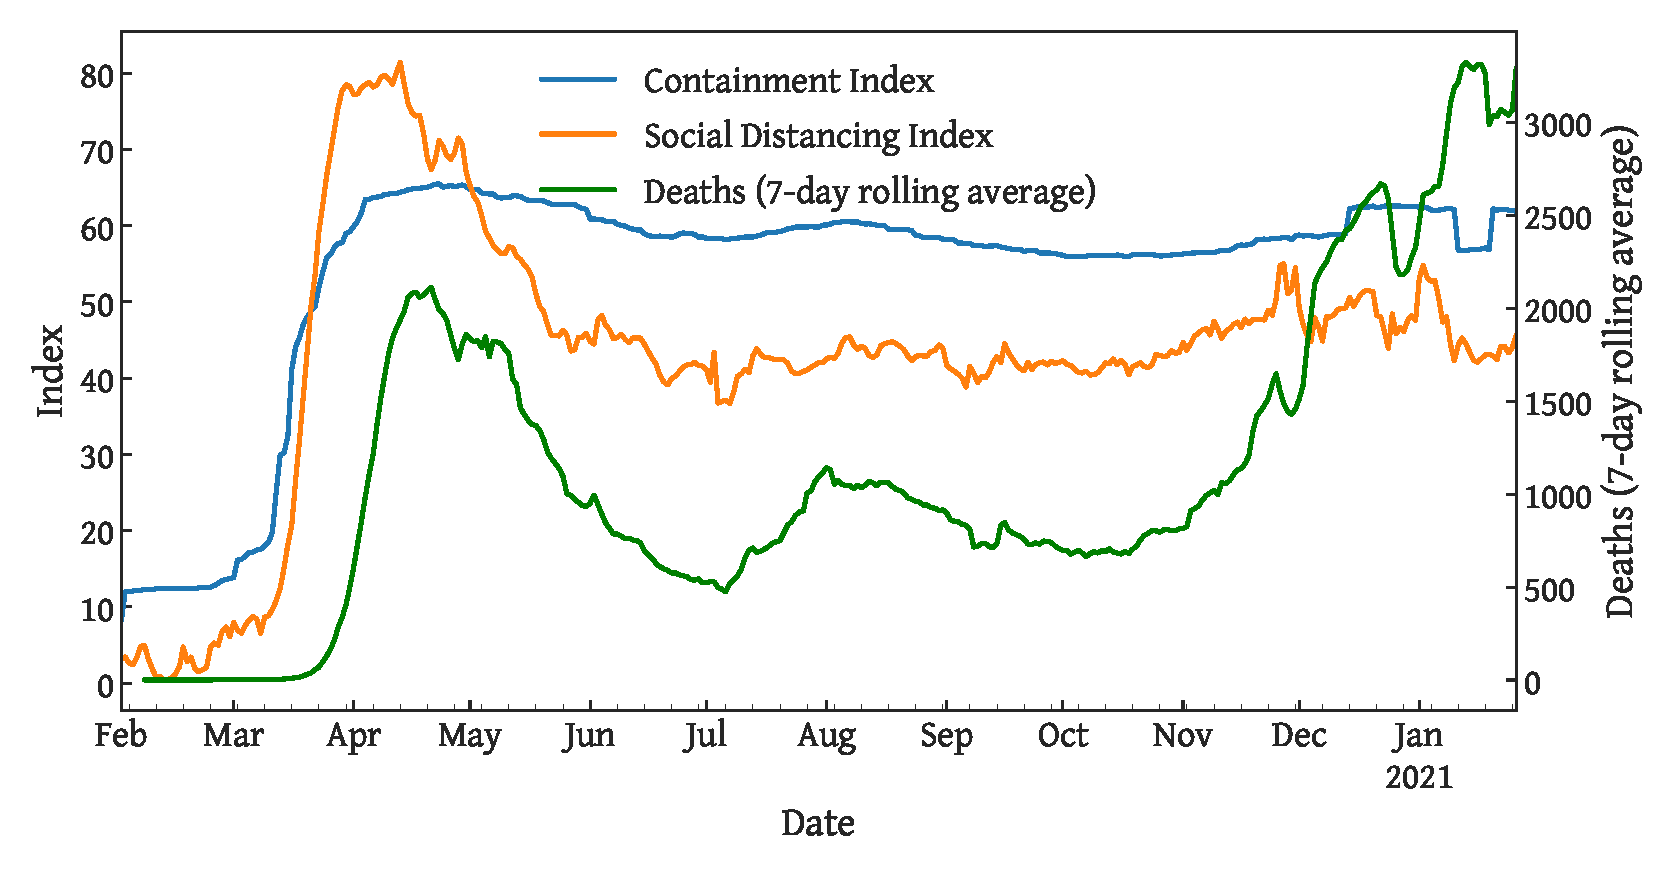
\includegraphics[width=0.8\textwidth]{us_mean_timeseries.eps}
    \caption{Daily time series of the OxCGRT Containment Health Index and our Social Distancing Index, both of which we average over all US states. For comparison, we plot the national daily death count, which we smooth using a 7-day rolling mean.}
    \label{fig:us_mean_timeseries}
\end{figure}

\begin{figure}[h!]
    \centering
    \includegraphics[width=0.9\textwidth]{sdi_containment_by_state.eps}
    \caption{Time series of the Containment Index and the SDI over the course of the pandemic, presented via heat map on a state-by-state basis across the US. Low containment/SDI is indicated in blue, whereas high containment/SDI is indicated in red.}
    \label{fig:sdi_containment_by_state}
\end{figure}

The mean curves mask significant heterogeneity across states. Figure~\ref{fig:sdi_containment_by_state} visualizes the containment index and SDI over the course of the pandemic across states. As in the aggregate picture, it is clear that social distancing relaxed much more than containment policies would indicate over the summer and fall of 2020. State-level plots comparing containment measures and the SDI over the pandemic are also available at \href{https://www.thesocialdistancingindex.xyz}{our website \ExternalLink} (more details below). 

Do containment measures and social distancing decrease COVID-19 spread? We will answer this question in a robust fashion below, but Figure~\ref{fig:sdi_containment_vs_infection} shows the correlation between the infection rate and SDI (top panel) and the infection rate and containment index (bottom panel) across states on several dates in 2020. This exploration of the data supports our intuition that public health measures can mitigate spread. Interestingly, for the final date in October, the containment measure appears less correlated with infection rate than the SDI. This may be due to differences in policy adherence; we study this with more rigor below.
%
\begin{figure}[h!]
    \centering
    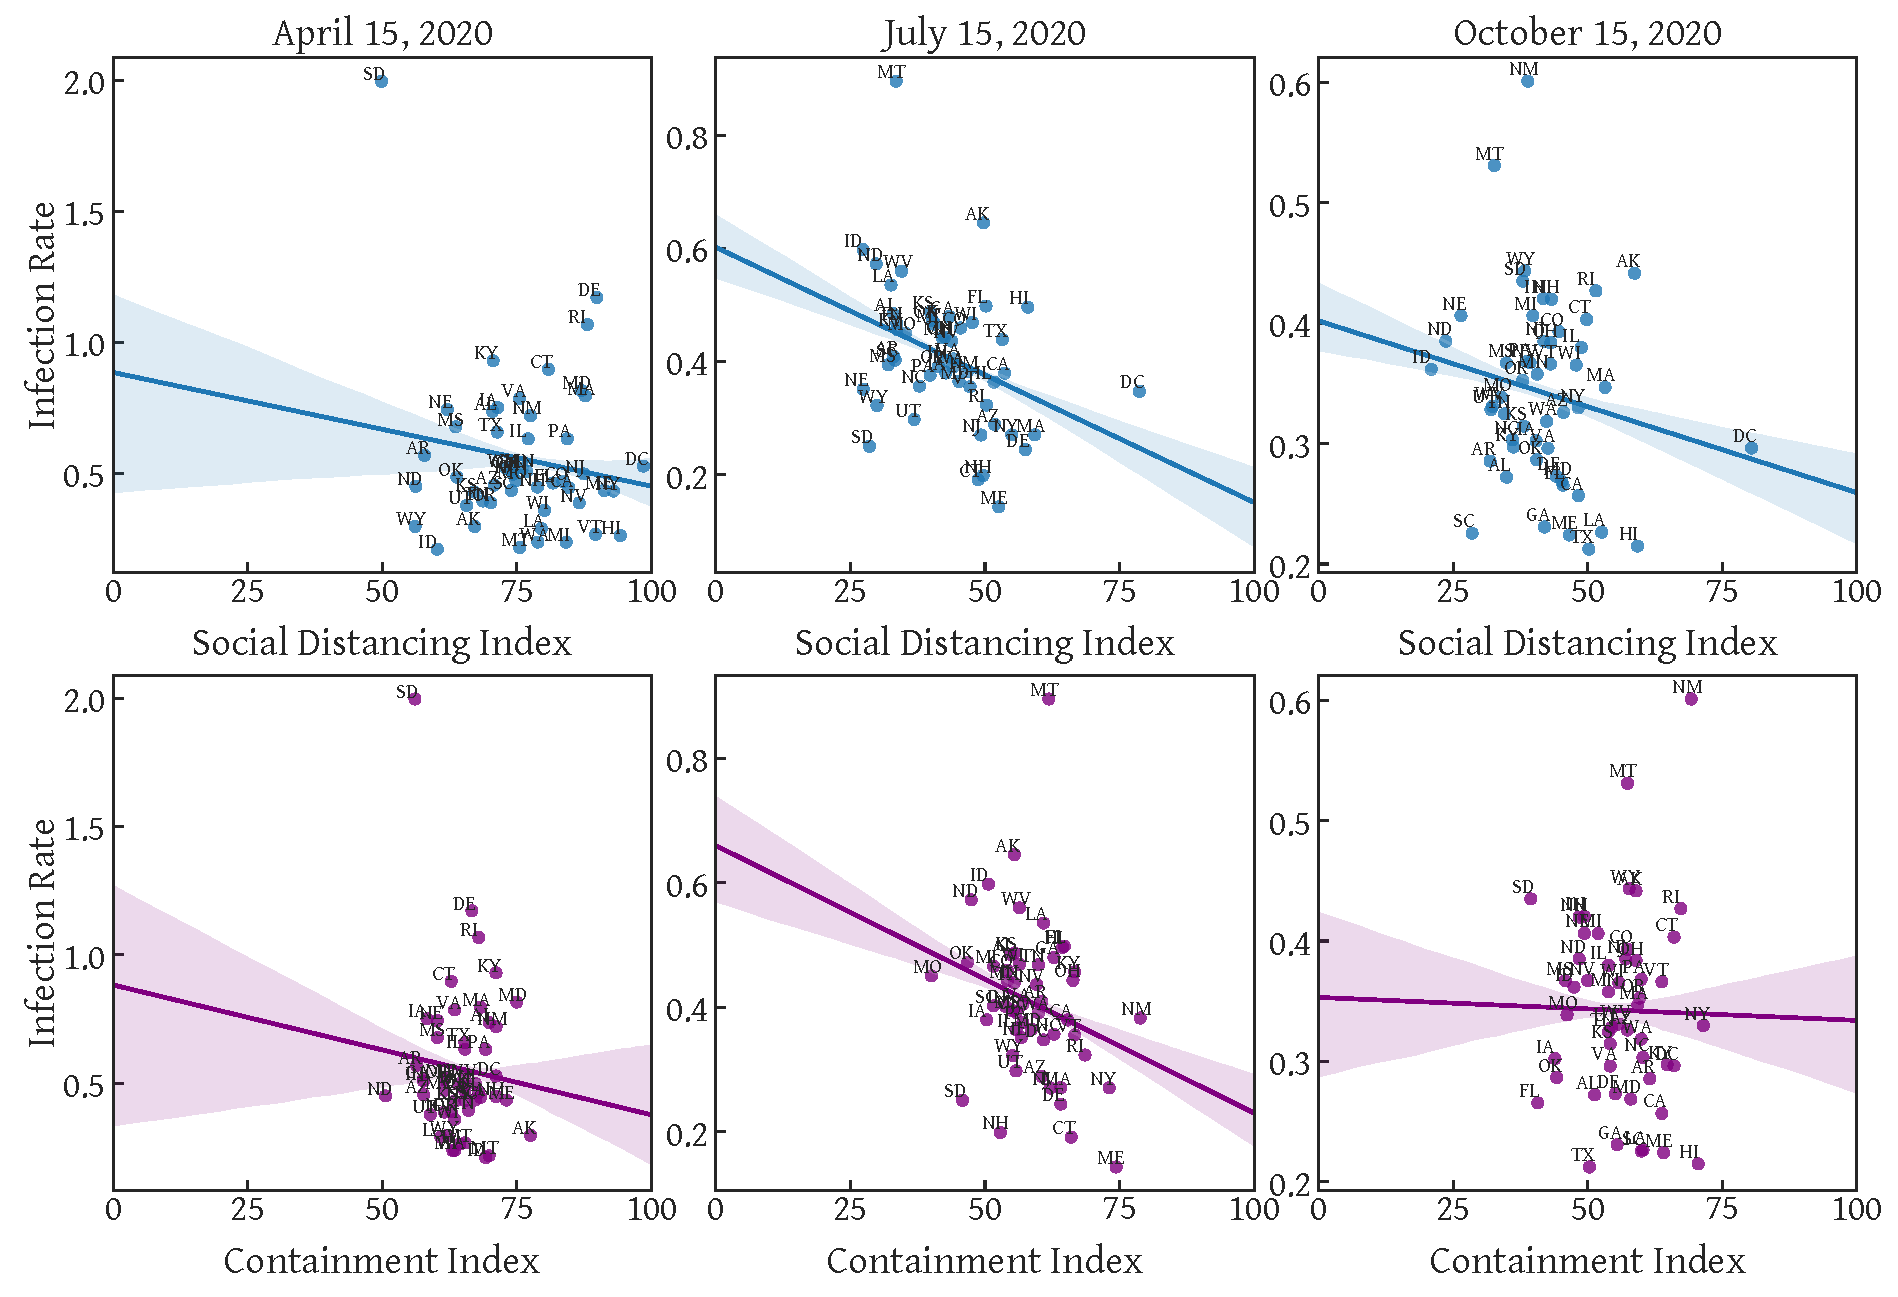
\includegraphics[width=0.9\textwidth]{sdi_containment_vs_infection.pdf}
    \caption{The infection rate (see Section~\ref{sssec:measures}) shown as a function of ({\it top}) the SDI and ({\it bottom}) the Containment Index on a state-by-state basis (shown with corresponding lines of best fit) on several dates during the pandemic.}
    \label{fig:sdi_containment_vs_infection}
\end{figure}

\subsection{Assessing the predictive power of the SDI}
\label{ssec:asso}

In this subsection, we show that our SDI outperforms other indicators in predicting the current and future spread rates of COVID-19 at the state level. We use the indicators listed in Section~\ref{sssec:measures} as measures of COVID-19 spread rates and calculate the degree to which using the SDI decreases the mean squared error of prediction estimates.

To most closely approximate a policy application of the index, we begin with a simple linear specification model to see how the SDI improves fit compared to using containment policies and previous case data for prediction. We fit a linear model to the data with controls only and then with the SDI. The advantage of this linear specification is that it also allows us to estimate the effect associated with increased social distance on spread rates; we expect this effect to be negative if social distancing mitigates transmission. The regression is
\[ \text{Virus Spread}_{i,t} = \alpha + \beta \, \text{SDI}_{i,t} + X'\gamma + \delta_j + \eta_k + \epsilon_{i,t}, \]
where $\delta_j$ and $\eta_k$ are month- and state-level fixed effects, and $X$ includes a number of controls such as containment measures and COVID-19 cases per capita in the last 14, 21, and 28 days.

Table~\ref{tab:reg_results} reports the results. As expected, an increase in the SDI is associated with a decrease in all measures of COVID-19 spread. The coefficient in all specifications is robust at the 1\% level (standard errors are clustered at the state-level). We find that including the SDI decreases the mean squared error of prediction between 6--12\% for most of our outcome variables. Interestingly, the degree to which the SDI decreases the mean squared error is greater for look-ahead variables, such as future case and death growth rates, and future infection rates. This supports our conjecture that SDI is a measure of current distancing, which should affect results over the following weeks. The SDI performs especially well when using $R_t$ (the viral reproduction number) as a measure of COVID-19 spread, decreasing the mean squared error of prediction by over 30\%. We test whether the increase in the fit provided by the SDI is significant using an $F$-test, finding $p$-values of $< 0.01$ for all specifications.

\begin{table}[h!]
\begin{tabular}{lcccccc}
\toprule
                          Outcome &  SDI &                                             95\% &  $R^2$ &  $R^2$ &  \% Decrease &       $F$-test \\
                           &  Estimate  &             Confidence Set                      &  Excl. SDI &  Incl. SDI & in MSE  &      $p$-value  \\
\midrule
                      Infection rate & -0.09447 &  [-0.1344, -0.0546] &        0.32 &        0.36 (+0.04) &          6.43\% &  $<0.01$ \\
         Weekly case growth & -0.09574 &    [-0.1365, -0.0550] &        0.30 &        0.35 (+0.05) &          6.29\% &  $<0.01$ \\
                Infection rate, 7 days ahead & -0.11072 &   [-0.1370, -0.0844] &        0.25 &        0.35 (+0.10) &          12.49\% &   $<0.01$ \\
   Weekly case growth, 7 days ahead & -0.11290 &   [-0.1390, -0.0868] &        0.23 &        0.33 (+0.10) &          12.48\% &  $<0.01$ \\
 Weekly death growth, 14 days ahead & -0.04601 &  [-0.0620, -0.0300] &        0.25 &        0.32 (+0.08) &          9.09\% &  $<0.01$ \\
 Weekly death growth, 21 days ahead & -0.04591 &  [-0.0569, -0.0349] &        0.19 &        0.28 (+0.09) &          10.90\% &  $<0.01$ \\
                               $R_t$ & -0.01086 &   [-0.0125, -0.0092] &        0.46 &        0.64 (+0.18) &          34.80\% &   $<0.01$ \\
                            $R_t$, 7 days ahead & -0.010230 &   [-0.0116, -0.0088] &        0.39 &        0.59 (+0.20) &          32.82\% &   $<0.01$ \\
\bottomrule
\bottomrule
\end{tabular}
\caption{Linear specification of the SDI effect on various COVID-19 spread measures. Estimates are reported from the base specification and standard errors are clustered at the state level. The $F$-test tests whether an unrestricted model including SDI improves predictive power over a restricted model excluding SDI.}
\label{tab:reg_results}
\end{table}

For robustness, we vary the controls, $X$, included in the specification and plot the results in Supplementary Figure~\ref{fig:sdi_containment_coefficients}. The coefficient estimated for the SDI is stable across all four specifications for each outcome variable. In particular, the magnitude of the coefficient on the SDI remains similar in regressions including or omitting the measure of containment policy. This supports our hypothesis that the true level of social distancing in practice provides valuable information beyond the stated containment policies.

We perform a similar exercise for the measure of policy containment measures, shown in the second panel of Figure~\ref{fig:sdi_containment_coefficients}. We notice that the coefficient on containment decreases in magnitude once the SDI is included in the specification, which suggests that the SDI contains valuable information about the true adherence to containment policies. However, both coefficients are significant across specifications, which suggests that both measures should be used in combination by policymakers for prediction.

\subsection{Application 1: Lockdown fatigue}
\label{subsec:fatigue}

A central question in decision-making during the COVID-19 pandemic is how effective containment policy is in reducing contact and thus reducing transmission. We showed that social distancing is indeed predictive of lower spread rates in the above section; now, we consider how effective policy is in increasing social distancing.

We use an event study framework with a differences-in-differences approach. We look at dates when the OxCGRT measure of state containment policy increased by five or more points --- we interpret this increase as an indicator that a state significantly increased containment measures on that date (there are 257 such events in the data). We then calculate the change in the SDI in that state before the policy and for 30 days after the policy implementation. If policy is effective at increasing social distancing behavior, we should expect a rise in the SDI following the policy change.

In order to isolate the effects of the policy, we then control for the contemporaneous increase in social distancing by other states that did \textit{not} have a change in policy over the same period. Our outcome is thus how much \textit{excess social distancing} was promoted by the lockdown policy,
\[ \text{SDI}_{s,t} - \text{SDI}_{s,0} = \alpha_t + \beta_t \times 1\{ \text{Policy change at $t=0$} \},  \]
where $s$ represents the state, $t$ denotes the time lag in days from the event, $\alpha_t$ is a fixed effect for the date, and $\beta_t$ is the size of the policy effect. We also report the average effect of a policy change on the SDI over the 30 days following the policy implementation (calculated as $\frac{1}{30} \sum_{t=0}^{30} \beta_t$). Standard errors are calculated via bootstrap resampling.

\begin{figure}[h!]
    \centering
    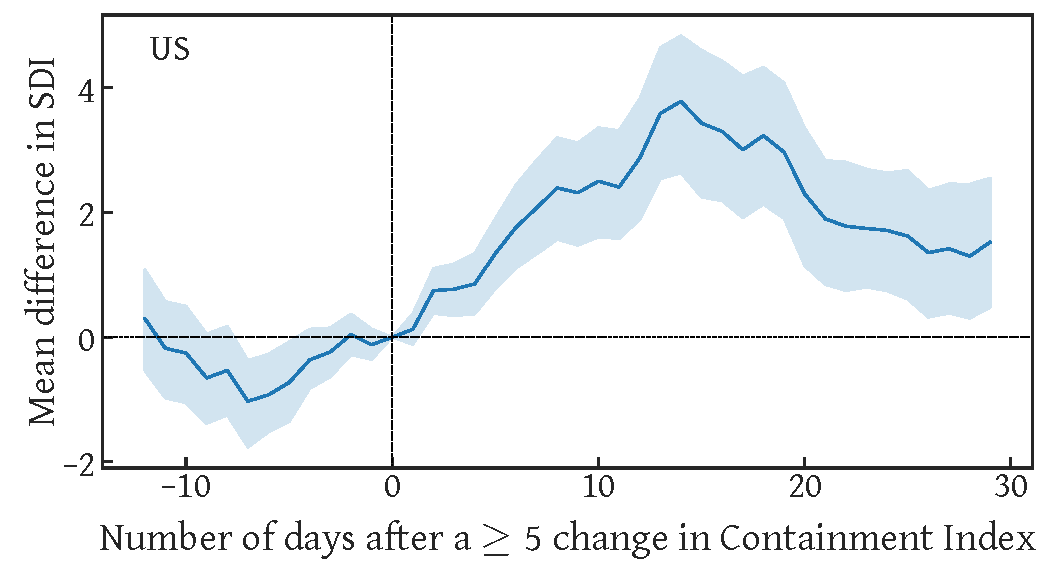
\includegraphics[width=0.5\textwidth]{impulse_response_all.pdf}
    \caption{The impulse response of the SDI in US states following an increase in the Containment Index of at least five points. The mean is taken over all such occurrences over the course of the pandemic and the shaded region denotes the 95\% confidence interval.}
    \label{fig:impulse_response_all}
\end{figure}

Figure~\ref{fig:impulse_response_all} shows the impulse response of excess social distancing following a five or greater point increase in containment measures over the whole sample. We see that an increase in containment policies results in a significant increase in social distancing: the SDI for states with a policy measure increases about four points at the peak of the response (about 12 days after the policy change). On average, the increase in containment policy results in a two point increase in the average social distancing in the 30 days following the policy.

\begin{figure}[h!]
    \centering
    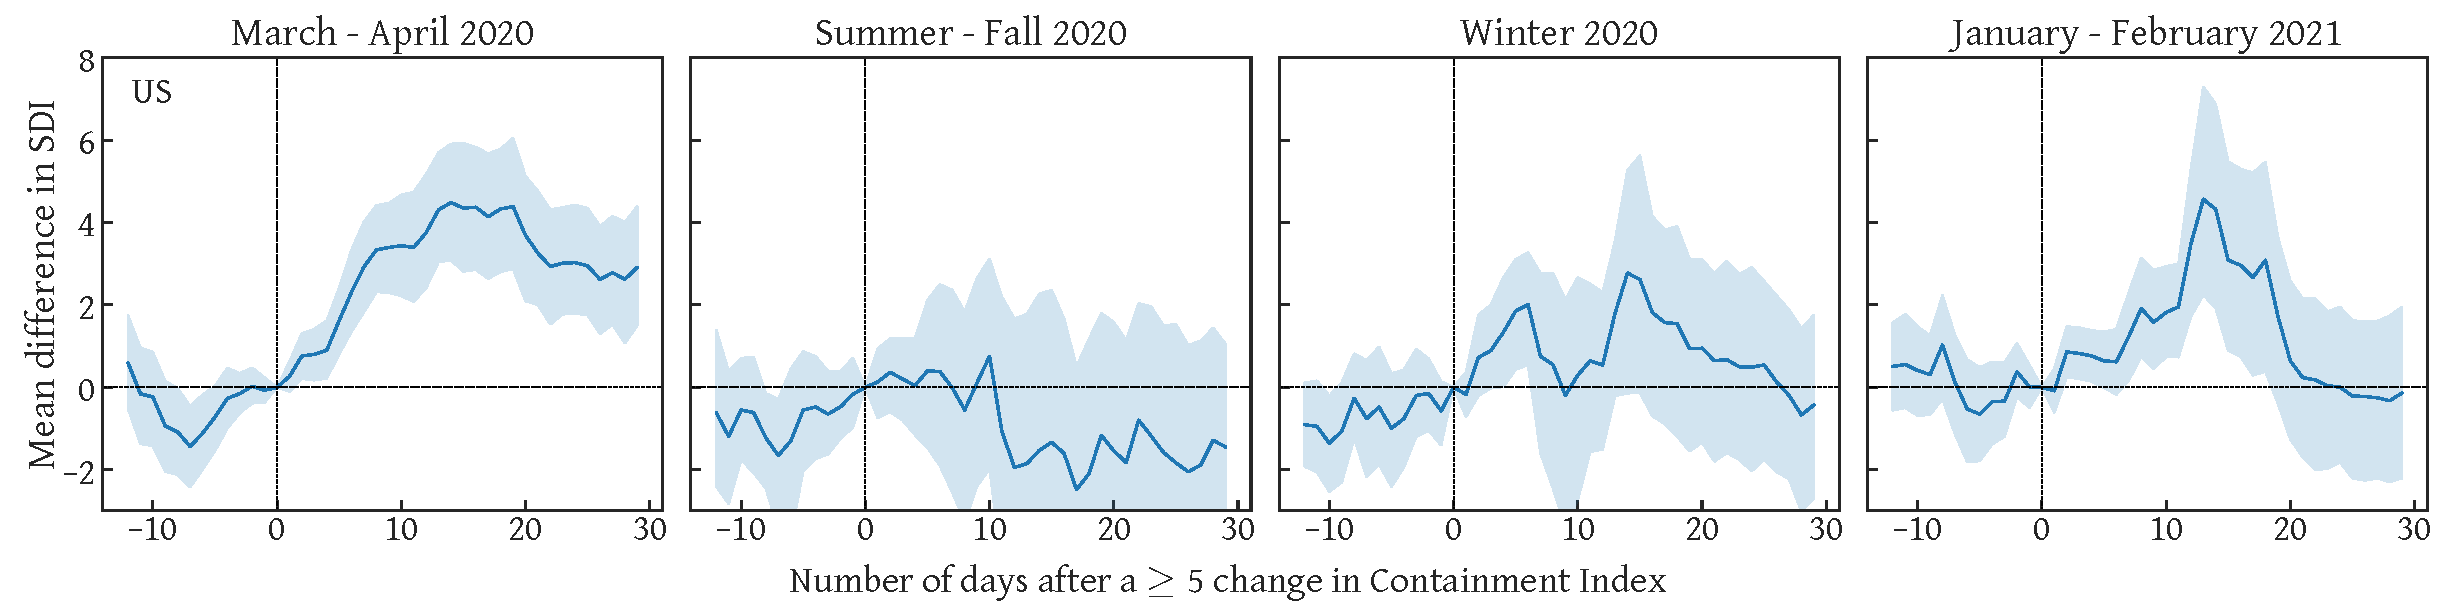
\includegraphics[width=\textwidth]{impulse_response_date.pdf}
    \caption{The impulse response of the SDI in US states following an increase in the Containment Index of at least five points. The sample is split into four time periods, such that the mean is taken over all such occurrences in a given period and the shaded region denotes the 95\% confidence interval within that period.}
    \label{fig:impulse_response_date}
\end{figure}

We then break the data into four subsamples to look at policy effectiveness over time: March--April 2020, May--September 2020, October--December 2020, and January--February 2021. Figure~\ref{fig:impulse_response_date} shows the impulse responses and Table \ref{tab:impulse_effect} reports confidence intervals on the mean effect on social distancing in the 30 days following the policy change.

The results show significant \textit{policy fatigue}: policy interventions in March--April 2020 had the greatest impact, increasing social distancing by 2.9 points on average after the policy. Later policy interventions were less effective. For instance, policies so far in 2021 increased social distancing by only 1.3 points in the 30 days after the policy, with the effect reverting about two weeks after the intervention. We cannot meaningfully discern the effects of lockdown policies in the summer or winter of 2020 from zero. To contextualize these results, recall that an increase in the SDI by one point is associated with a decrease in the fractional infection rate and case growth rate by 0.09--0.11 and a decrease in the weekly death growth rate by about $0.05$.

\begin{table}[h!]
\centering
\begin{tabular}{lc}
\toprule
{Dates} & {Effect on SDI (30 day mean)}  \\
 & [95\% confidence set] \\
\midrule
Whole sample    & 2.0 ***   \\
 &  $[1.4, 2.6]$ \\
\midrule
March-April 2020     & 2.9 ***   \\
 & $[2.0, 3.8]$ \\
May-September 2020    & -1.0  \\
 & $[-3.0, 1.2]$ \\
October-December 2020    & 0.8    \\
 & $[-0.5, 2.1]$ \\
January-February 2021     & 1.3 **    \\
 & $[0.1, 2.4]$ \\
\bottomrule
\bottomrule
\end{tabular}
\caption{The effect of an increase in state containment policies on the SDI (30-day mean). Standard errors are calculated via bootstrap resampling.}
\label{tab:impulse_effect}
\end{table}

Next, we estimate the impact of lockdown fatigue on the effective post-lockdown $R_t$. Our methods are based on epidemiology research literature --- we apply the transmission curve of COVID-19 as estimated in \href{https://link.springer.com/article/10.1007/s10729-020-09504-6}{Kaplan (2020) \ExternalLink}.

Specifically, using Wuhan data, Kaplan (2020) estimates the transmission curve of an infected person to follow a gamma distribution over time with parameters $\alpha = 1.55$ and $\beta = 2.84$. The crucial parameter that epidemiologists and policymakers are concerned about, namely the viral reproduction number, $R_t$, is actually the integration of the area under the transmission curve.

We take these parameters and plot the transmission curve in the left panel of Figure~\ref{fig:R0}. Note that if the containment policy comes into effect right after virus detection and lasts ever since, then the transmission after the containment policy will be blocked entirely. However, if there is policy fatigue starting from around two weeks after the containment policy (like we have illustrated above), the later part of the transmission curve is not effectively blocked, which will create a difference in the post-lockdown $R_t$. The initial unblocked area simply reflects that the virus detection takes time after infection, which is estimated to be 5.7 days on average.

In the right panel of Figure \ref{fig:R0}, we show what the post-lockdown $R_t$ will be if we take into consideration the 14-day policy fatigue in comparison to the no-fatigue situation. The horizontal axis captures the adherence rate immediately following policy implementation. The blue curve shows the ``no-fatigue'' case, demonstrating that $R_t$ can be reduced to $<1$ as long as the adherence rate is at least 75\% initially. The red curve shows the ``policy fatigue'' case, where we assume that the adherence rate will drop by half after 14 days of implementation. Once this is taken into consideration, we see that the post-lockdown $R_t$ becomes much higher, such that we need at least a 90\% adherence rate initially in order to effectively control the spread of the virus. This comparison demonstrates that the policymakers need to be cautious about potential fatigue in order to reduce COVID-19 spread.

\begin{figure}[htb!]
	\centering
    \centering
    \begin{minipage}[t]{0.48\textwidth}
    \centering
    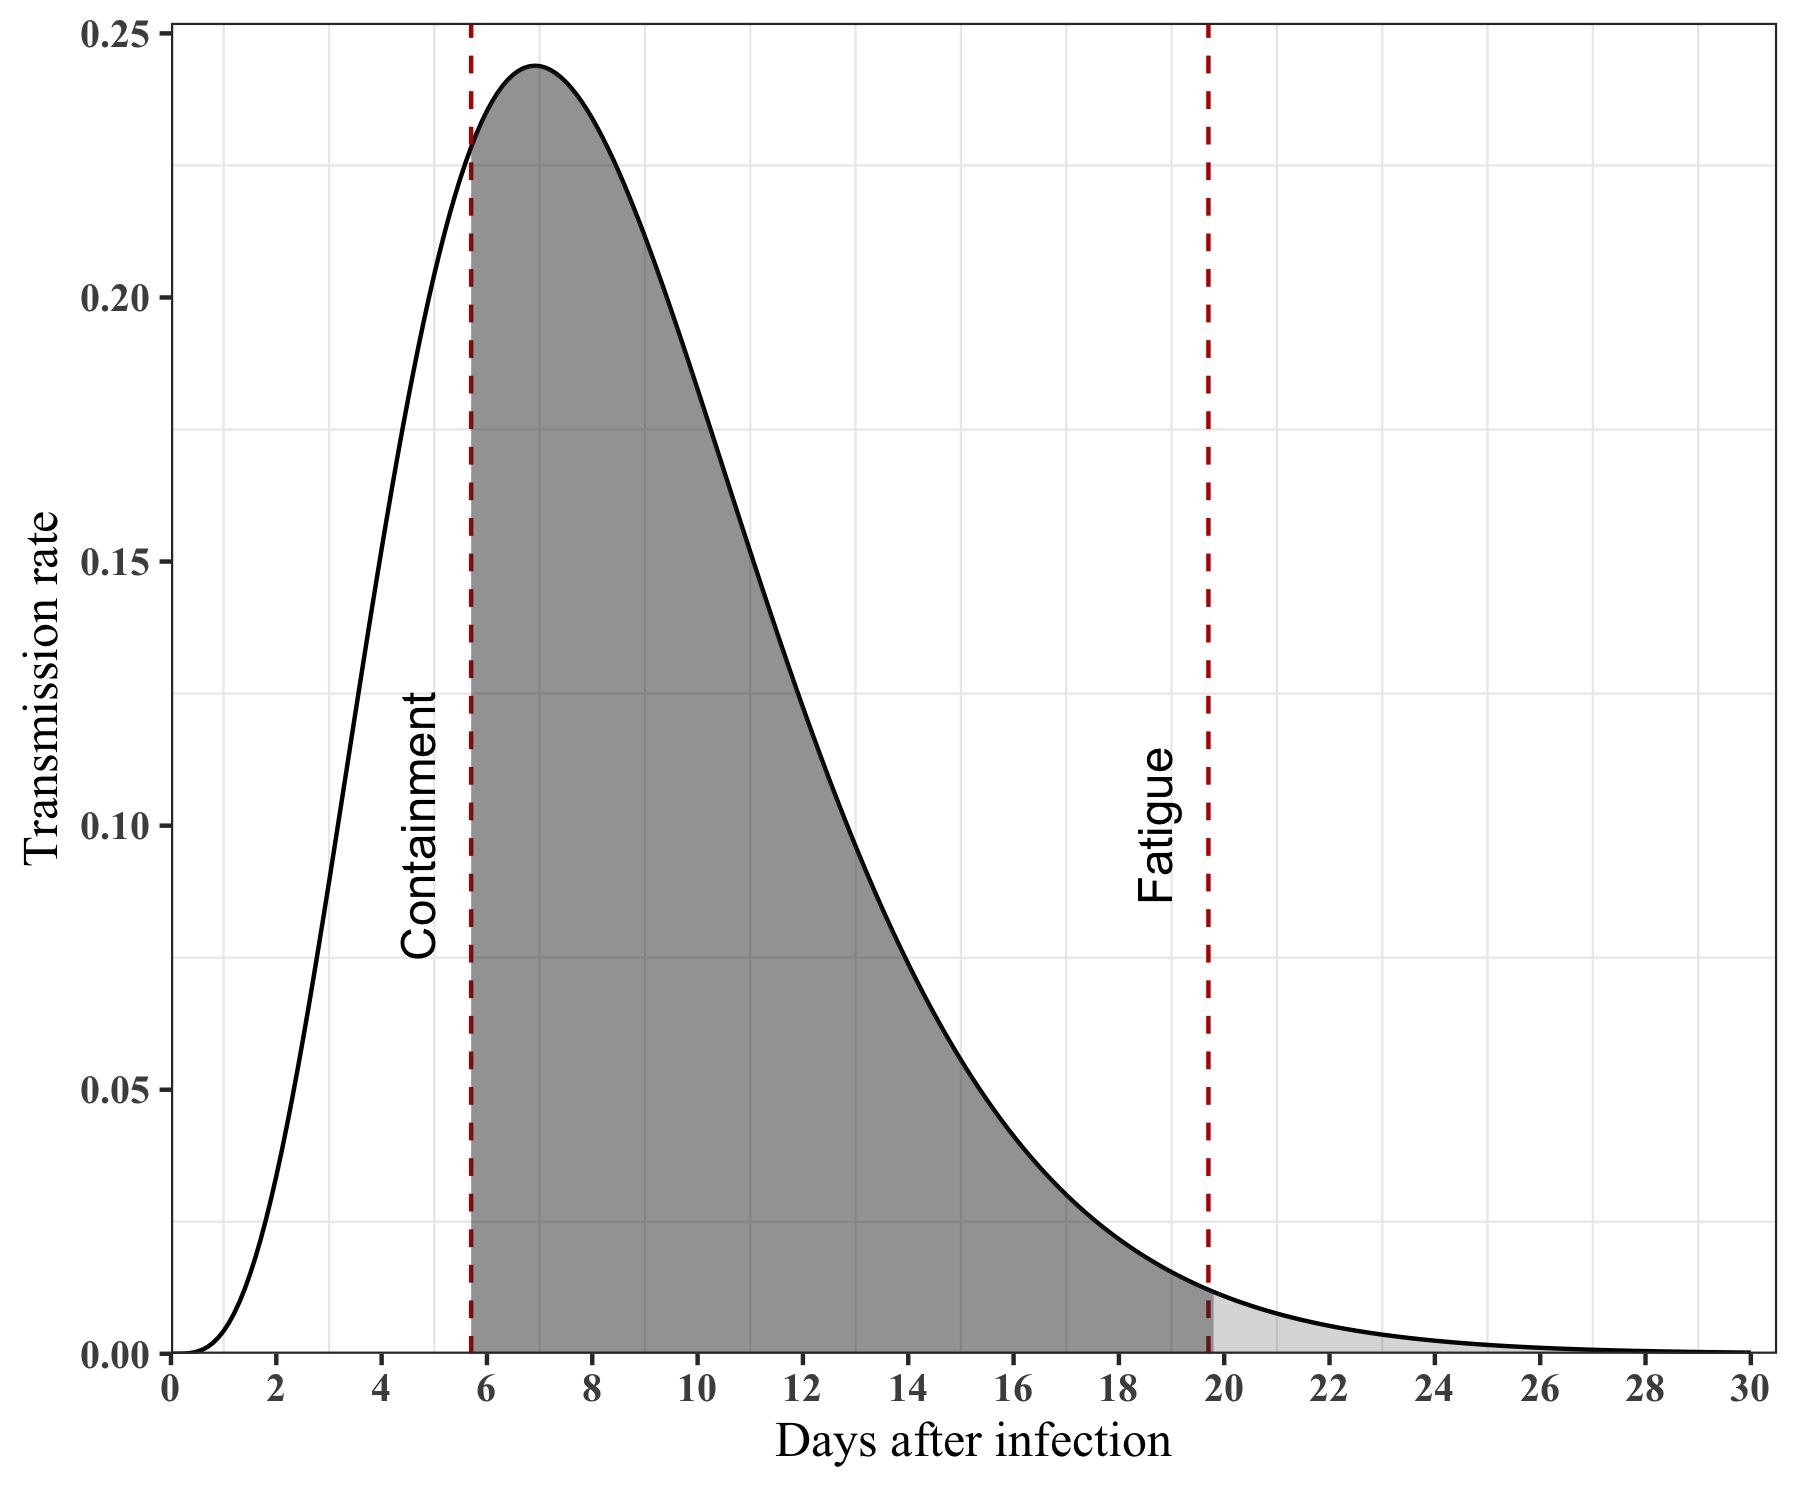
\includegraphics[width=8.3cm]{R0.png}
    \end{minipage}
    \hspace{1.5em}
    \begin{minipage}[t]{0.48\textwidth}
    \centering
    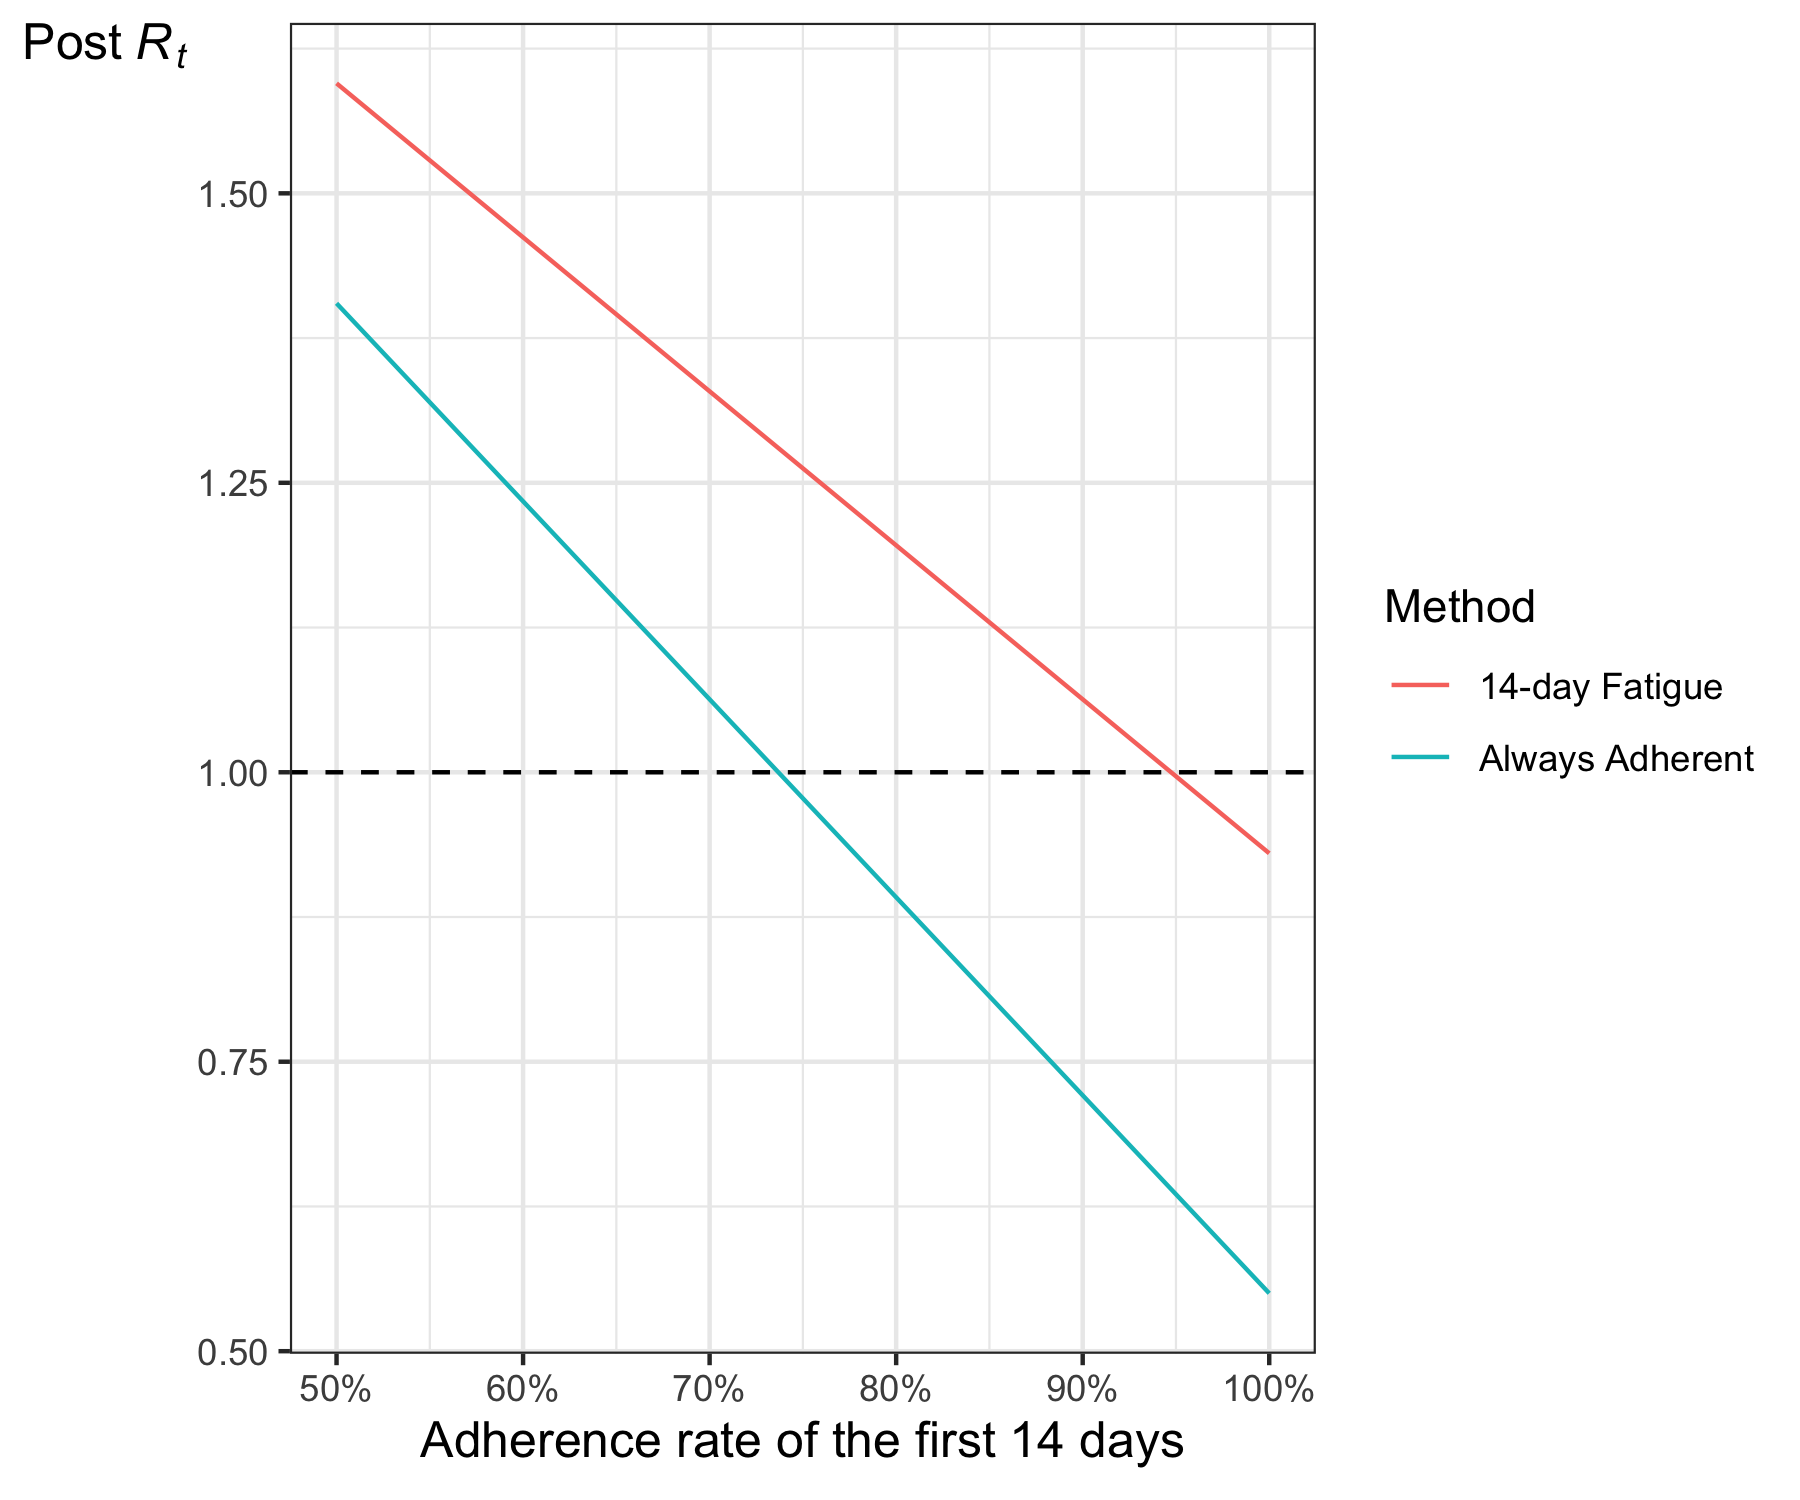
\includegraphics[width=8.3cm]{postR0.png}
    \end{minipage}
	\caption{\small The impact of policy fatigue on effective post-lockdown $R_t$.}
	\label{fig:R0}
\end{figure}

\subsection{Application 2: Policy adherence and political ideology}
%state political affiliation}
Figure \ref{fig:us_map} visualizes the average containment policy level and social distancing level from July 2020--present.\footnote{These measures began to stabilize around July 2020. We note that results remain qualitatively the same if earlier months are included as well.} Overall, states in the northeast and on the west coast tend to have higher magnitudes in both indices compared to states in the mid-west and south. 

\begin{figure}[h!]
    \centering
    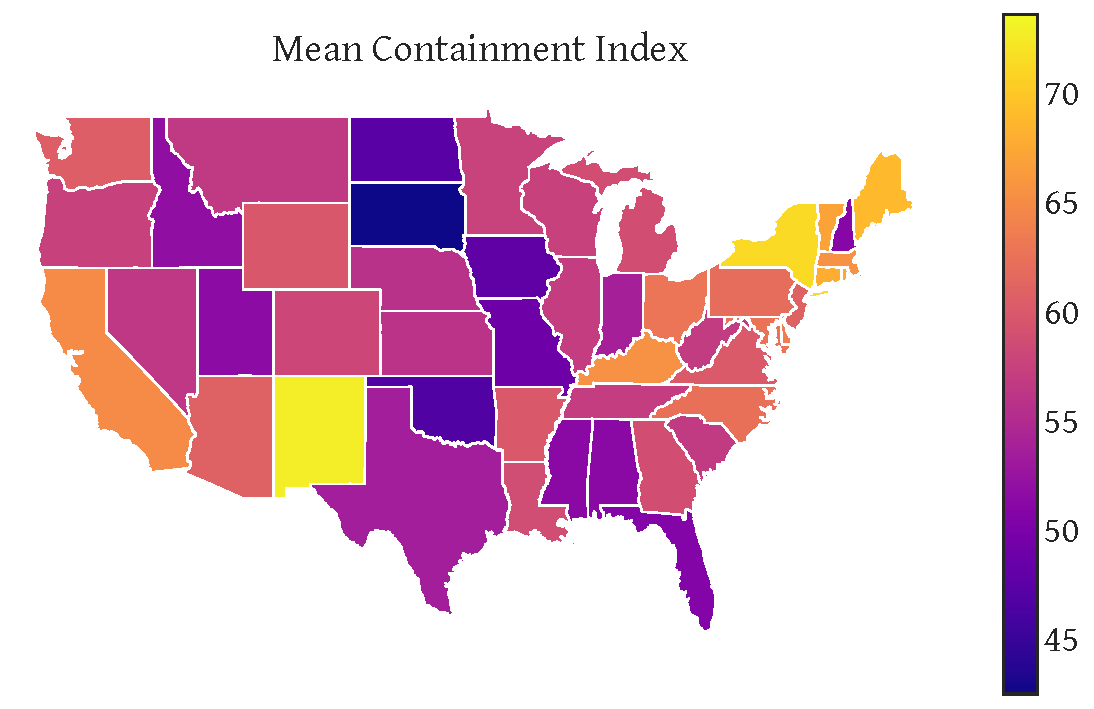
\includegraphics[width=0.47\textwidth]{mean_containment.pdf}
    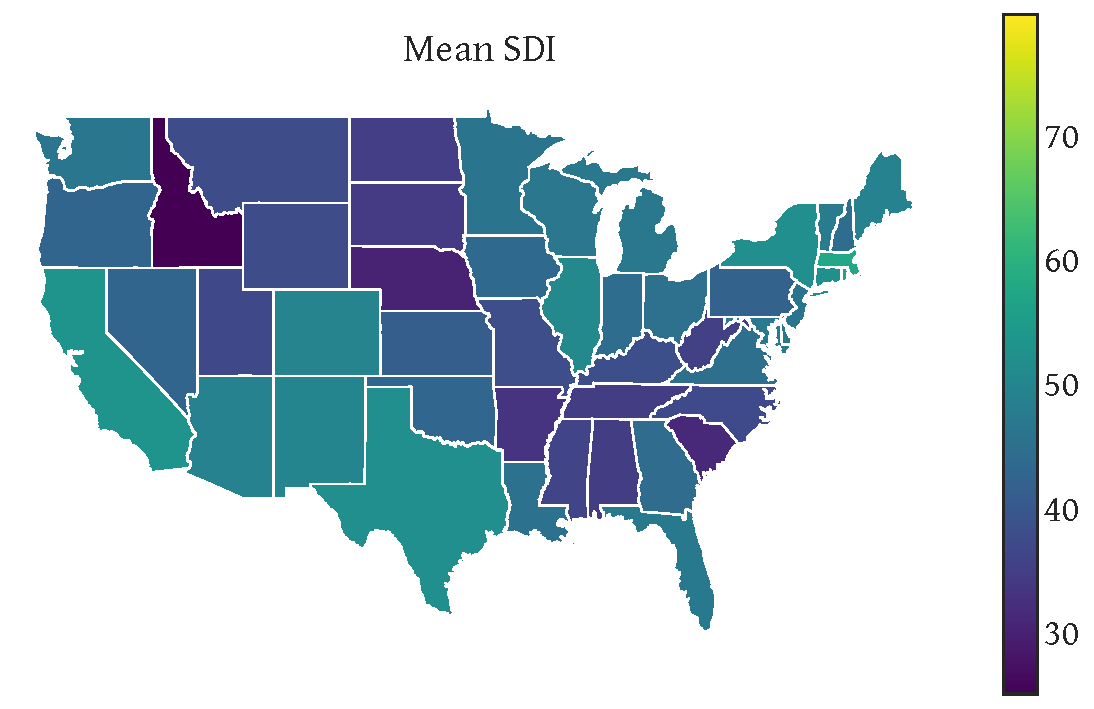
\includegraphics[width=0.47\textwidth]{mean_sdi.pdf}
    \caption{A visualization of the Containment Index and SDI averaged over the pandemic (from July 2020 onward) on a state-by-state basis on the continental US map.}
    \label{fig:us_map}
\end{figure}

What determines the heterogeneity of policy measures and social distancing across states? We hypothesized based on the state map visualizations that this heterogeneity may be related to various socioeconomic and political factors. We explore one dimension of this question by considering how state political affiliation affected the containment policies put in place and the subsequent adherence to them. We measure political affiliation by the political party of the state governor and the state's vote in the 2020 presidential election. 

We classified the 50 states based on the governor's party and voting outcome in the 2020 presidential election. We are interested in comparing the containment and social distancing strength across states belonging to the four categories: (Republican governor, voted for Trump), (Democratic governor, voted for Biden), (Republican governor, voted for Biden), and (Democratic governor, voted for Trump).

\begin{figure}[h!]
    \centering
    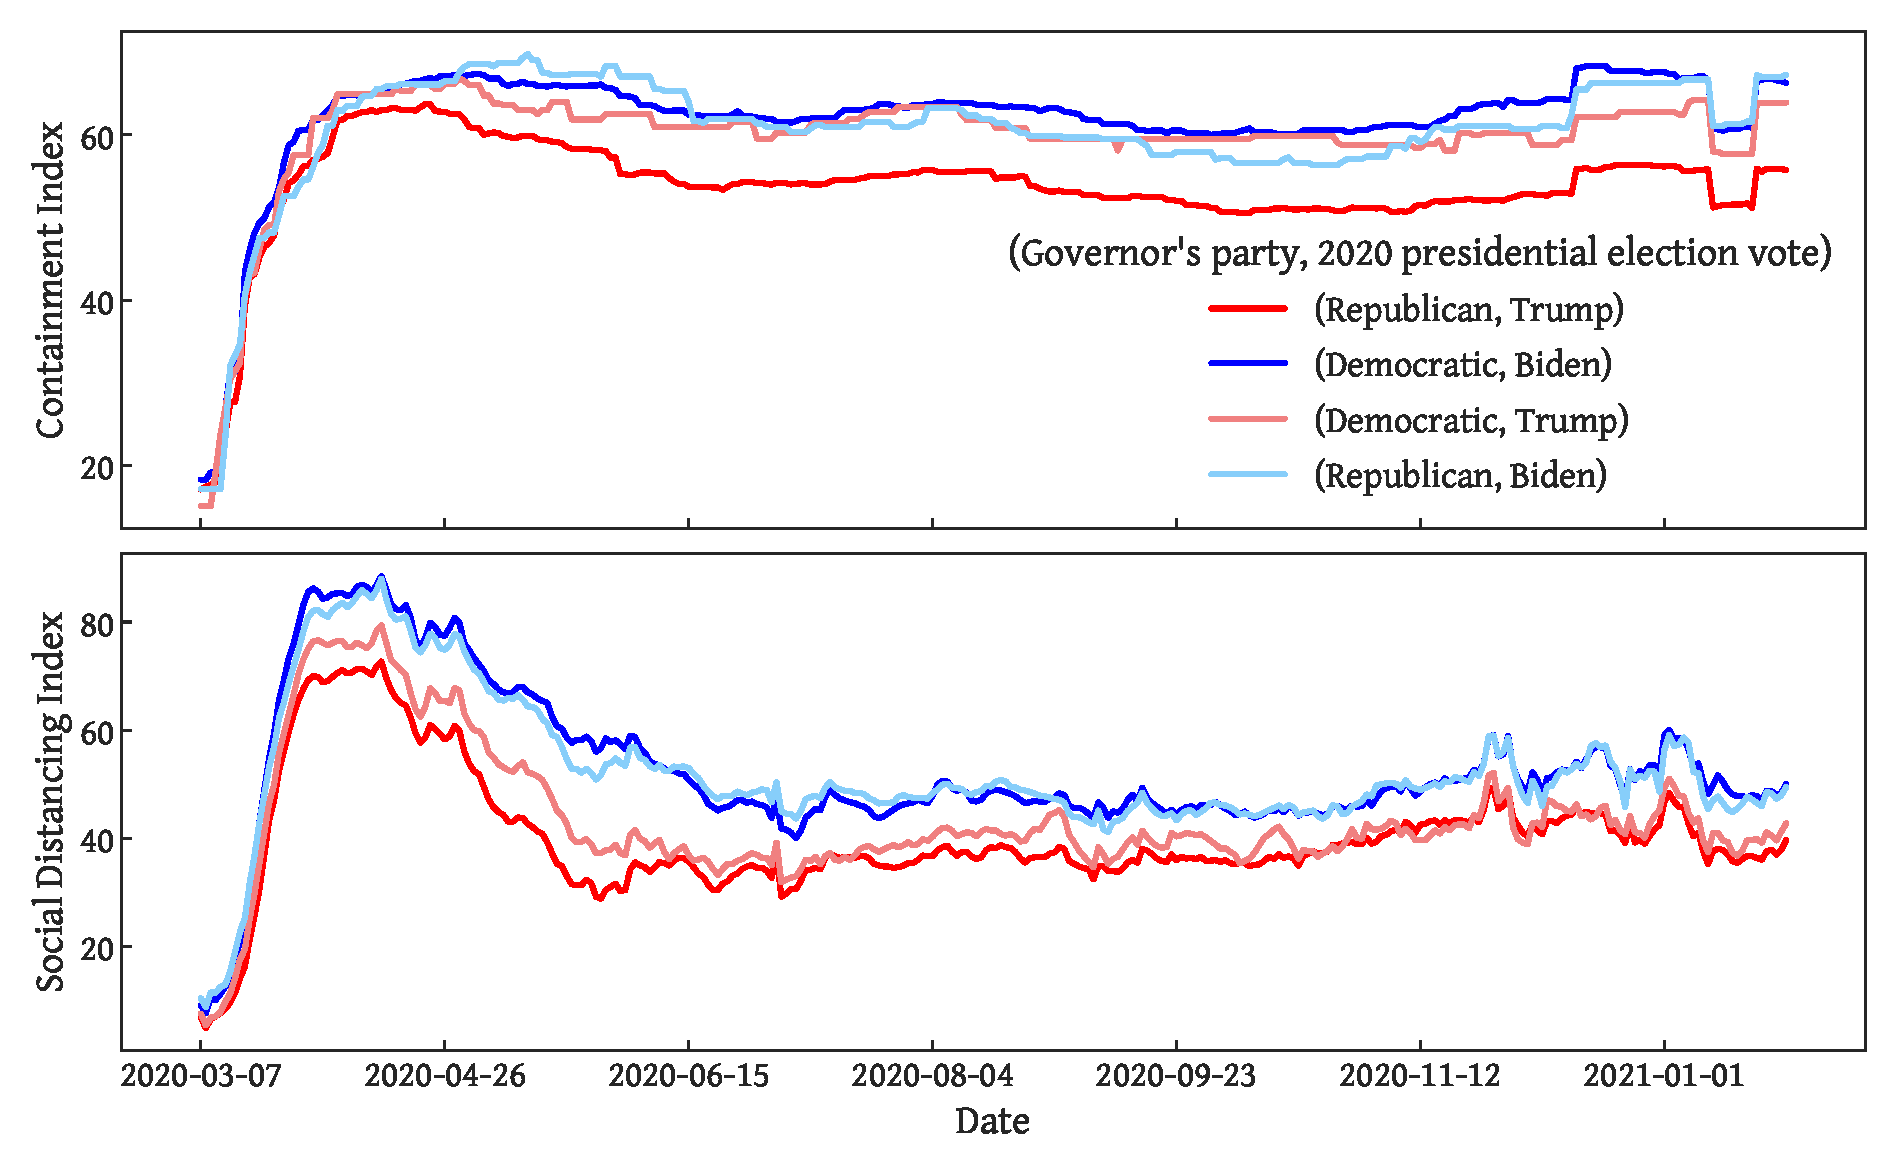
\includegraphics[width=\textwidth]{sdi_containment_repdem.eps}
    \caption{{\it Top}: Time series of the Containment Index averaged over states belonging to each one of the four categories based on the governor's political party and 2020 presidential election vote results. {\it Bottom}: Time series of the SDI averaged over states split into the same four groups.}
    \label{fig:sdi_containment_repdem}
\end{figure}

Figure \ref{fig:sdi_containment_repdem} shows the time series of containment policies and the SDI for each of the four groups. States with both a Republican governor and that voted for Donald Trump put less stringent containment measures in place than other states. Interestingly, states with Republican voting results have consistently lower SDI then those with Democratic voting results. The governor's party, in contrast, does have an effect on social distancing with SDI being higher when the governor is Democratic, but this effect is small compared to the voting outcome feature. We summarize these results using an ``adherence ratio'', which is simply the ratio between the SDI and the containment index. We take the mean adherence ratio (from July 2020 onward) separately over all states in each of the four groups and present the results in Table~\ref{tab:adherence_ratio_by_party}. The states that voted for Trump have the lowest adherence overall. In particular, states with a Democratic governor and a 2020 vote for Trump have a low SDI and higher containment, resulting in an adherence value far below the national average (0.67 compared to 0.75). On the other hand, Biden-voting states with Republican governors maintain a high SDI in the presence of a lower containment, resulting in the highest adherence ratio on average.

We learned a few lessons from this analysis. The political belief of the local citizens and the governor has a visible influence on the containment measures being taken. The fact that the presidential election voting outcome rather than the governor's party is a driving factor for social distancing practices reveals a serious gap between the policy itself and people's responses to it. People's political beliefs seem to shape their responses to the pandemic, and public health policymakers should take this factor into account when disseminating disease control instructions to the citizens.

\begin{table}[h!]
\centering
\begin{tabular}{cccc}
\toprule
& & \multicolumn{2}{c}{Governor's party} \\
& & {Republican} & {Democratic}  \\
\multirow{2}{*}{2020 vote} & {Trump} & 0.72 & 0.67 \\
& {Biden} & 0.79 & 0.77 \\
\bottomrule
\bottomrule
\end{tabular}
\caption{The mean {\it adherence ratio}, defined as the ratio between the SDI and the Containment Index, taken from July 2020 onward for states that fall into each of the four categories determined by the governor's party affiliation and the state's 2020 presidential election vote. For comparison, the mean adherence ratio over the entire US is 0.75.}
\label{tab:adherence_ratio_by_party}
\end{table}

\section{Open questions}

Our results also open several new avenues for research. From a policy perspective, an open question remains about the optimal stringency of lockdown policy: lockdowns reduce spread, but excessively severe policies may induce too much fatigue over time. Using our data, future research can assess how designing lockdown policy for a ``marathon'' rather than a ``sprint'' impacts longer horizon outcomes. There is also an opportunity to better understand the determinants of distancing behavior, as driven by norms, media, politician messaging, and other factors.  

To aid in these efforts, we launched a website making our index publicly available to researchers and policymakers at \href{https://www.thesocialdistancingindex.xyz}{The Social Distancing Index \ExternalLink}. Visitors can look at the time series of SDI and containment measures across states, explore a map of social distancing by state over time, and download our data and this report. We hope to add more functionality, for instance to automate the whole process in this study and update the index on a daily basis. The hope is that this website can alert decision makers of potential outbreaks when the SDI falls and give real-time feedback on policy effectiveness.

%We created a web application that automates the analysis in this study available at: \href{https://www.thesocialdistancingindex.xyz}{The Social Distancing Index \ExternalLink}. More specifically, the app automatically extracts data from the various sources we listed to compute the SDI, updated on a daily basis. It analyzes and visualizes case numbers, policy stringency, and the SDI by states and countries in real time. It will alert decision makers of potential outbreaks when the SDI goes down, and gives real time feedback on the current policy. Furthermore, it encourages people to consistently adhere to the social distancing rules.

\section*{References}
\begin{hangingpar}
Chetty, Raj, John N. Friedman, Nathaniel Hendren, Michael Stepner, and The Opportunity Insights Team (2020). \textit{The economic impacts of COVID-19: Evidence from a new public database built using private sector data.} National Bureau of Economic Research, Working Paper No. 27431.
\end{hangingpar}
%
\begin{hangingpar}
Hale, Thomas, Sam Webster, Anna Petherick, Toby Phillips, and Beatriz Kira (2020). \textit{Oxford COVID-19 Government Response Tracker.} Blavatnik School of Government.
\end{hangingpar}
%
\begin{hangingpar}
Kaplan, Edward H. (2020). \textit{Containing 2019-ncov (Wuhan) coronavirus.} Health Care Management Science 23.3: 311-314.
\end{hangingpar}
%
\begin{hangingpar}
Systrom, Kevin, Thomas Vladek and Mike Krieger (2020). \textit{Rt.live}. GitHub repository, \href{https://github.com/rtcovidlive/covid-model}{https://github.com/rtcovidlive/covid-model \ExternalLink}.
\end{hangingpar}

%\pagebreak
\appendix
\part*{Supplementary Materials}

\section{European Union analysis}\label{app:eu}
\renewcommand{\thefigure}{A\arabic{figure}}
\setcounter{figure}{0}

In order to generalize our findings to locations outside of the US, we also carry out analysis using data from countries in the European Union (EU). Due to the data quality and availability, the analysis on the EU countries is done at the weekly level.

\subsection{Social Distancing Index (SDI) for the EU countries}

\paragraph*{Data sources:}
Firstly, we collect a comprehensive list of social mobility data for every country in the European Union. Specially, the data we gather include:

\begin{itemize}
\item \href{https://www.google.com/covid19/mobility/}{Google Community Mobility Reports \ExternalLink}: Available since February 2020 for different countries around the globe. We download the data directly from their website and select the data related to the 27 countries in the European Union and the U.K. Specifically, the data contains six different daily time series that measure the daily mobility relative to the baseline: retail and recreational, grocery and pharmacy, transit, workplace, parks, and residential.\footnote{We exclude the ``residential mobility'' series in Google Mobility as it captures the time people spend \textit{at home} instead of outside.}
\item \href{https://covid19.apple.com/mobility}{Apple Mobility Trends Reports \ExternalLink}: Apple provides mobility tracking data since January 2020, which we download directly from their website. Apple collects these data based on requests submitted through Apple Maps, offering three daily time series that measure mobility: transit, walking, and driving.
\item \href{https://ansperformance.eu/data/}{EU Airline Traffic Data \ExternalLink}: EuroControl’s Aviation Intelligence Unit collects daily departure and arrival flight data for each airport in Europe. We compress the data to the country-day level by summing up the number of departure and arrival flights for all the airports in each country. We then calculate the percentage change of the departure and arrival flights for every day in 2020 and 2021 compared to the same day in 2019.
\end{itemize}

\paragraph*{SDI Construction --- Principal Components:} Following the same procedure that was used to study the United States in the main text, we clean and merge the data that we have collected, take the first principle component of all of the mobility variables (which is ten time series in total), and transform it into the SDI.

\begin{figure}[h!]
    \centering
    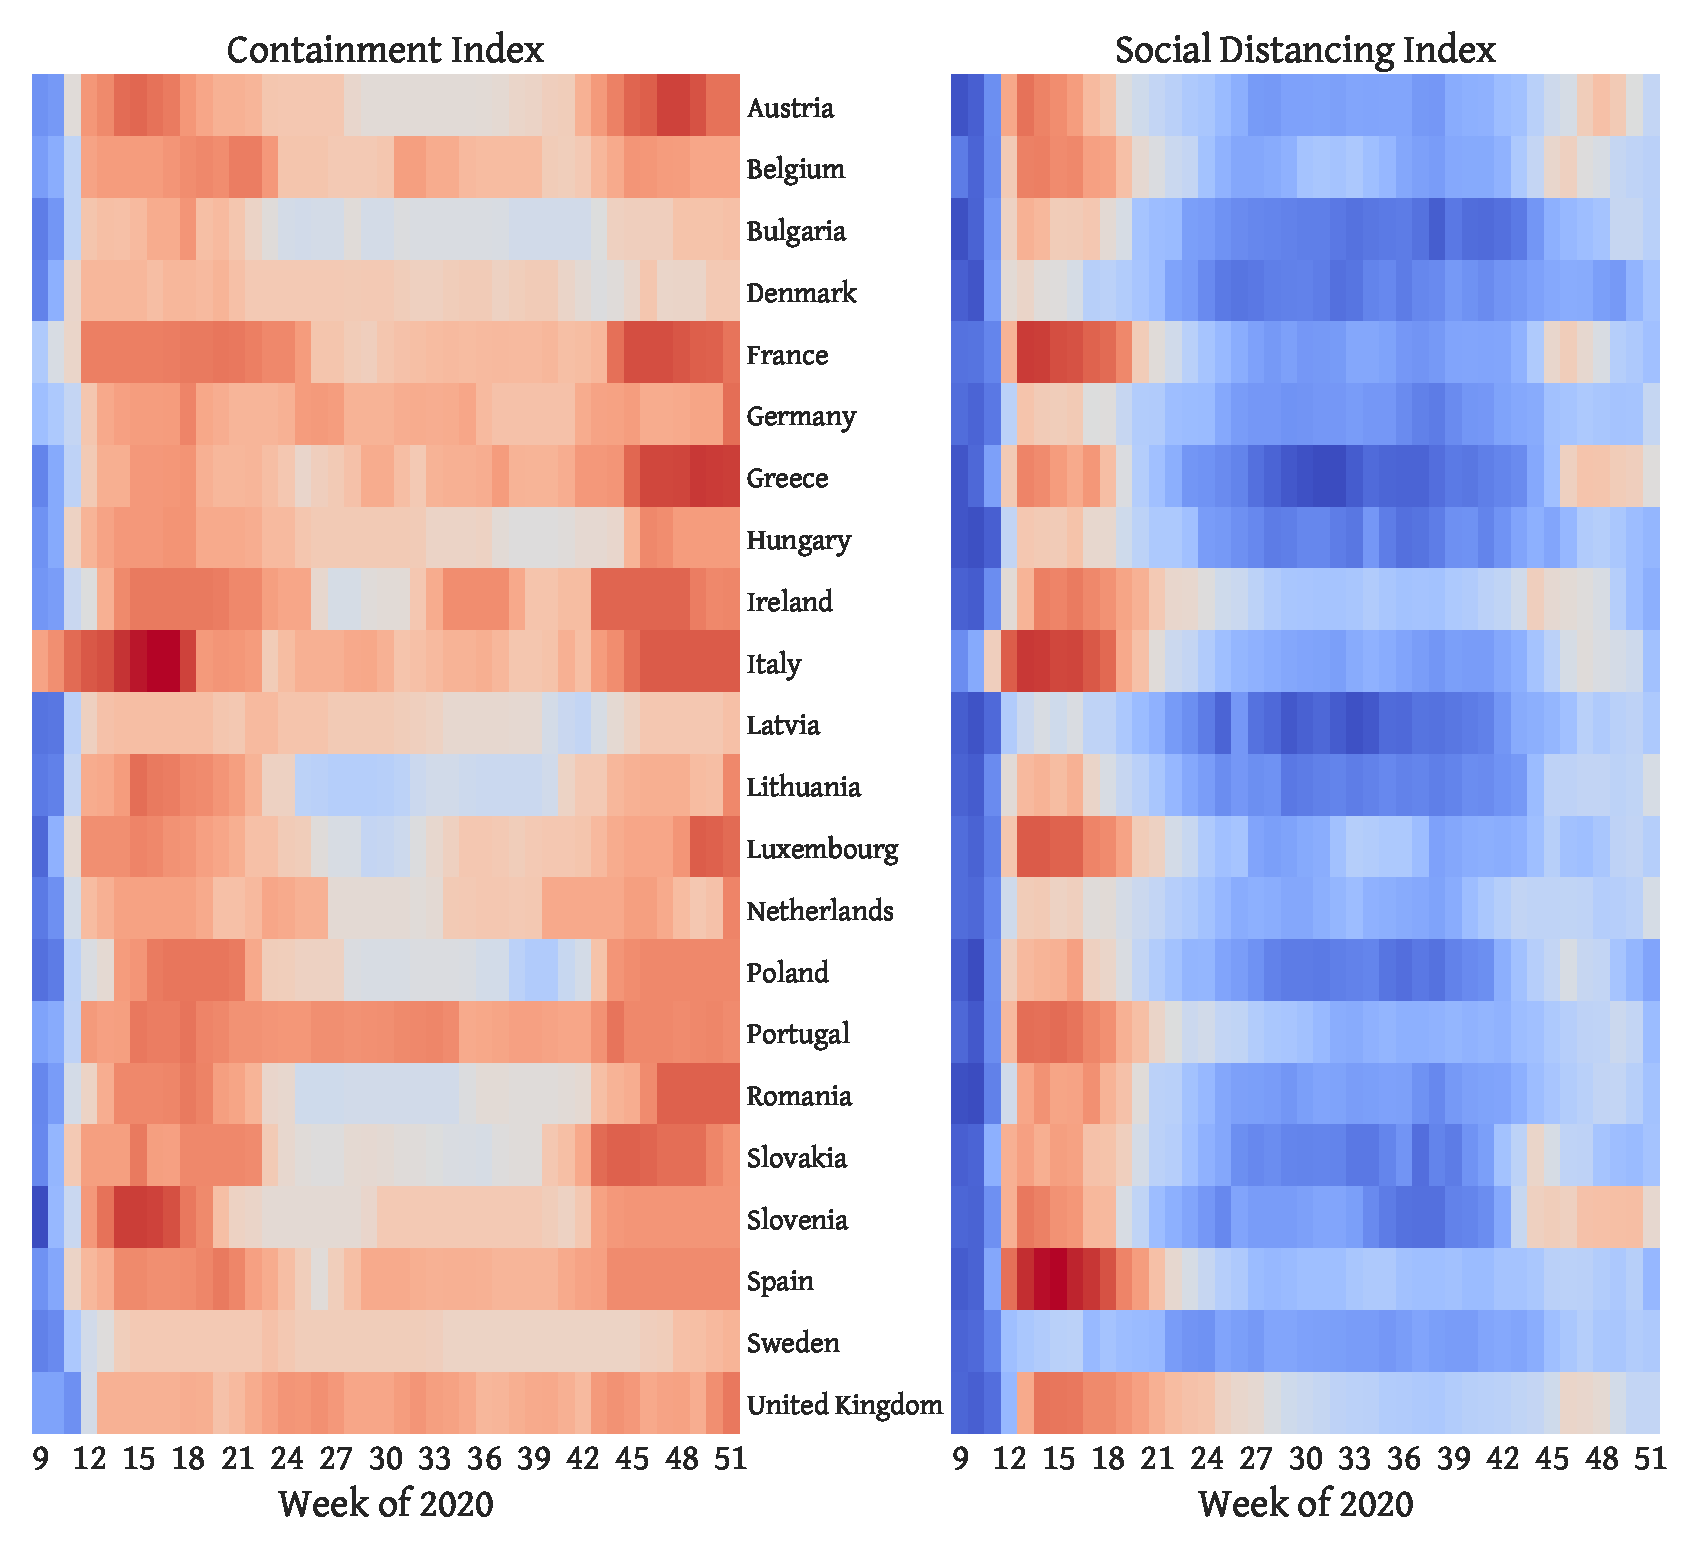
\includegraphics[width=0.9\textwidth]{eu_sdi_containment_by_country.eps}
    \caption{Time series of the Containment Index and the SDI over the course of the pandemic, presented via heat map on a country-by-country basis across the EU. Low containment/SDI is indicated in blue, whereas high containment/SDI is indicated in red.}
    \label{fig:eu_sdi_containment_by_country}
\end{figure}

\subsection{Association between the SDI and case spread}

In this subsection, we examine the associations among the government containment policies, the SDI, and virus spread. First, as Figure~\ref{fig:eu_sdi_containment_by_country} illustrates, for almost all countries in the EU, the SDI bounced back several weeks after lockdowns began whereas the containment policies did not change much. Next, we compare the predictive power of the government containment policies and the SDI on the future virus spread. Specifically, the future virus spread is captured in several different measures, as in Section \ref{ssec:asso}: the infection rate, the case growth rate, and the death growth rate. We run the same regressions as in Section \ref{ssec:asso}, but
%$$\text{Virus\ Spread}_{i,t} = \alpha + \beta_0 \text{Containment}_{i, t-1}+ \beta_1 \text{SDI}_{i, t-1} + \delta_j + \eta_k + \varepsilon_{i,t}$$
now $\eta_k$ represents a regional fixed-effect (we divide Europe into four regions: western Europe, eastern Europe, northern Europe, and southern Europe).

We summarize the regression results in Table \ref{tab:EU}. For all measures of virus spread, we observe that the SDI has better explanatory power (as reflected by the $R^2$) compared to the government containment measure. Furthermore, the $R^2$ uniformly increases for the regressions that include the containment measure when we add the SDI. This evidence indicates that in European countries, the actual social mobility instead of the government policy ``by the paper'' also has more impact on the future spread of the virus.

\begin{table}[h!]
\centering
\begin{tabular}{lccccccccccc}         							
\hline
\noalign{\smallskip}
\hline
\noalign{\smallskip}                                        
& \multicolumn{3}{c}{Panel A: $\text{Infection \ rate}_t$} &   &	 \multicolumn{3}{c}{Panel B: $\text{Case \ growth \ rate}_t$} & 	& \multicolumn{3}{c}{Panel C: $\text{Death \ growth \ rate}_{t+2}$}	\\	
\cmidrule(lr){2-4}\cmidrule(lr){6-8} \cmidrule(lr){9-12} 
$\text{Containment}_{t-1}$	& 	-0.0095	 & 	 &-0.0055	& &-0.0140	 &	 & -0.0084 & 	& 	-0.0043 &	 & 0.0026 \\
	&	[0.0014]	& 	& [0.0016] & 	&[0.0025]	 &	 & [0.0026]& 	&[0.0047] &	 & [0.0052]	\\
$\text{SDI}_{t-1}$	&	&	-0.0055 		& -0.0065	&&	&-0.0112	 & -0.0091 & 	 & &-0.0097 & -0.0104 \\
	&	&[0.0016]	& [0.0019]&  &	&[0.0017] & [0.0019]& 		 & &[0.0020]	 & [0.0025]	\\
\\
$R^2$ & 0.2384  & \textbf{0.2545} & \textbf{0.2617} &		&0.1806 & \textbf{0.1956} & \textbf{0.2042} & &0.1031  & \textbf{0.1148} &  \textbf{0.1139} \\
\hline\noalign{\smallskip} 
\hline\noalign{\smallskip}                                        			
\end{tabular}
\caption{The association between the SDI and several metrics of virus spread.}
\label{tab:EU}
\end{table}

\subsection{Lockdown fatigue}

Our next analysis on the EU countries revolves around using the impulse response function methods as outlined in Section \ref{subsec:fatigue}. We define the impulse as a sudden increase in the government containment measure,\footnote{For our EU analysis, a sudden increase is defined as an increase of the containment index by more than 8\%, which is the 85th percentile of the government containment policy variations over time.} and then examine the change of the SDI following this increase. The difference here is that we use a time horizon of five weeks before and 15 weeks after. Due to the smaller number of data points, we divide the analysis into two periods (instead of four periods as was performed for the United States): the first half of 2020 and the second half of 2020. Figure \ref{fig:eu_impulse_response_date} captures the impulse response over time.


\begin{figure}[htbp]
    \centering
    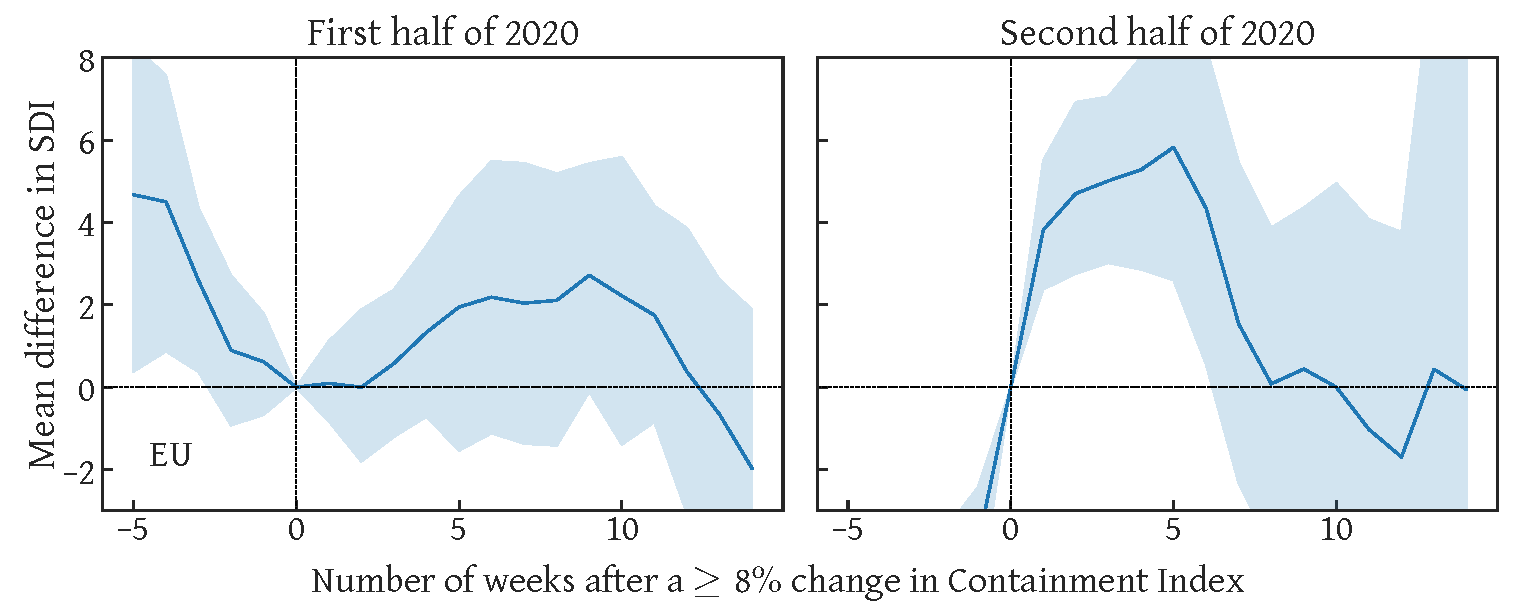
\includegraphics[width=0.8\textwidth]{eu_impulse_response_date.pdf}
    \caption{The impulse response of the SDI in EU countries following an increase in the Containment Index of at least eight percent relative to its previous value. The sample is split into two time periods, such that the mean is taken over all such occurrences in a given period and the shaded region denotes the 95\% confidence interval within that period.}
    \label{fig:eu_impulse_response_date}
\end{figure}

Similar to the US, we observe that the SDI first jumped up after the increase of government stringency. However, as time passed by, the ``stay-at-home fatigue'' began to emerge, with a turning point happening at around two months after the onset of the lockdown policy. After about three months of increased lockdown, the policy effect on social distancing was nearly nonexistent and \textit{even slightly negative}. We observe a stronger effect for the second half of 2020, with a reversal occurring at around a month after policy implementation. This makes intuitive sense: when the virus bounced up after summer and another round of lockdowns were carried out, people became more easily fatigued. Our estimated length of time for fatigue to show up is comparable to that of the US, i.e., one to two months.

All of these results above consistently show that the findings and policy suggestions we have laid out for the United States can also be generalized to countries around Europe.

\pagebreak
\section{Supplementary figures}
\renewcommand{\thefigure}{B\arabic{figure}}
\setcounter{figure}{0}

\begin{figure}[h!]
    \centering
    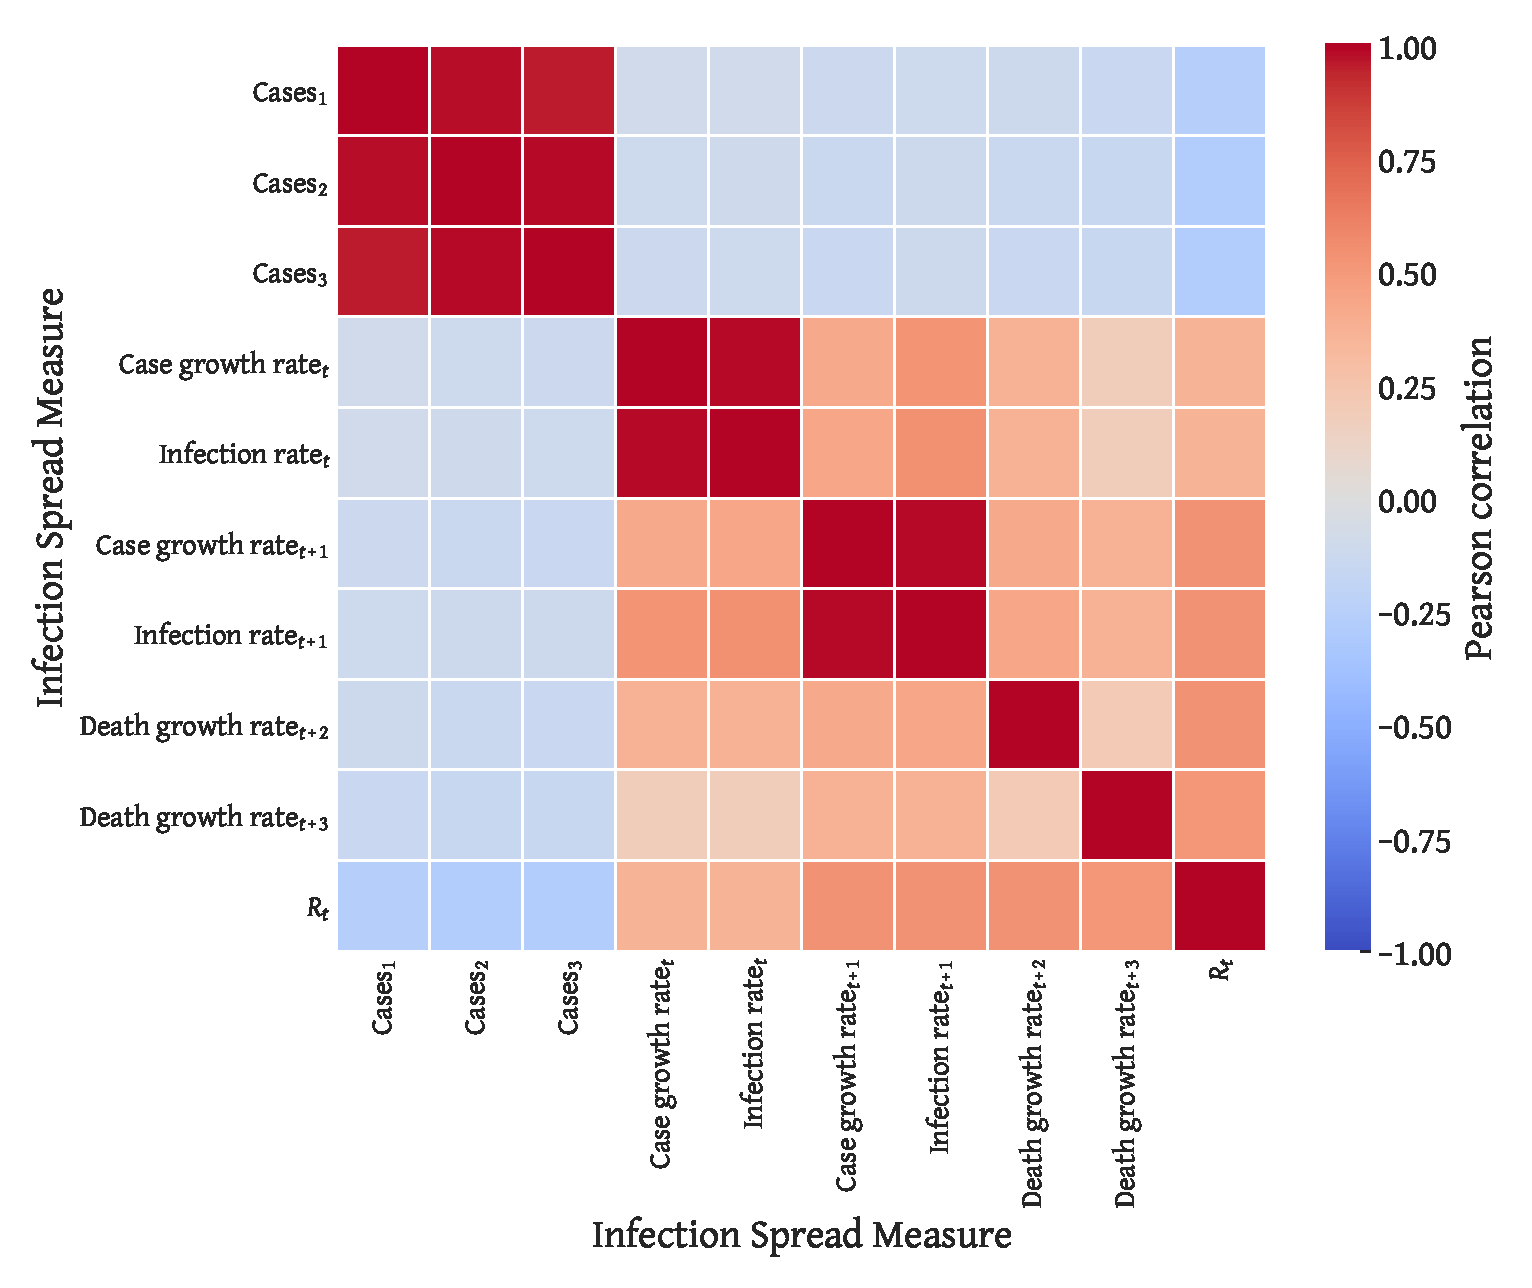
\includegraphics[width=0.75\textwidth]{corr_outcomes.eps}
    \caption{The pairwise correlation between each of our infection spread measures over the course of the pandemic across all US states. See Section~\ref{sssec:measures} for precise definitions of each measure.}
    \label{fig:corr_outcomes}
\end{figure}

\begin{figure}[h!]
    \centering
    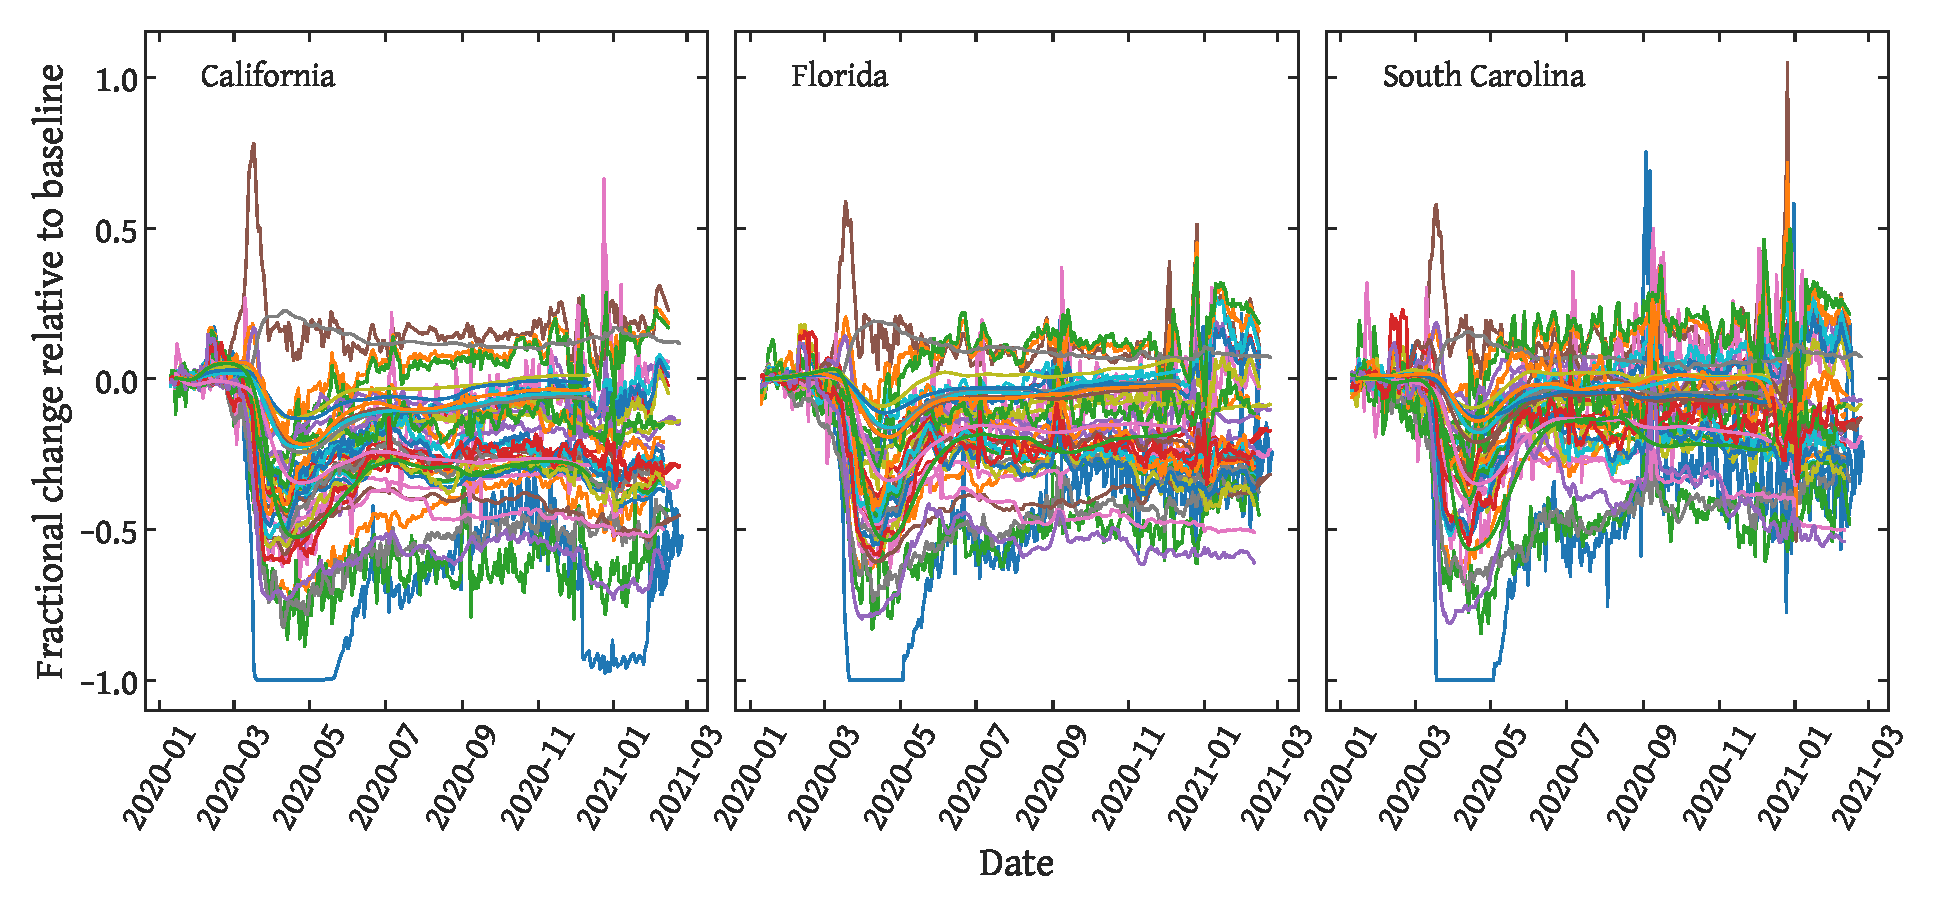
\includegraphics[width=0.9\textwidth]{raw_indicators.eps}
    \caption{Time series of the raw mobility indicators used to construct our Social Distancing Index, each expressed in terms of its fractional year-of-year change relative to 2019. See Section~\ref{sssec:extdata} for a description of the data and the sources.}
    \label{fig:raw_indicators}
\end{figure}

\begin{figure}
    \centering
    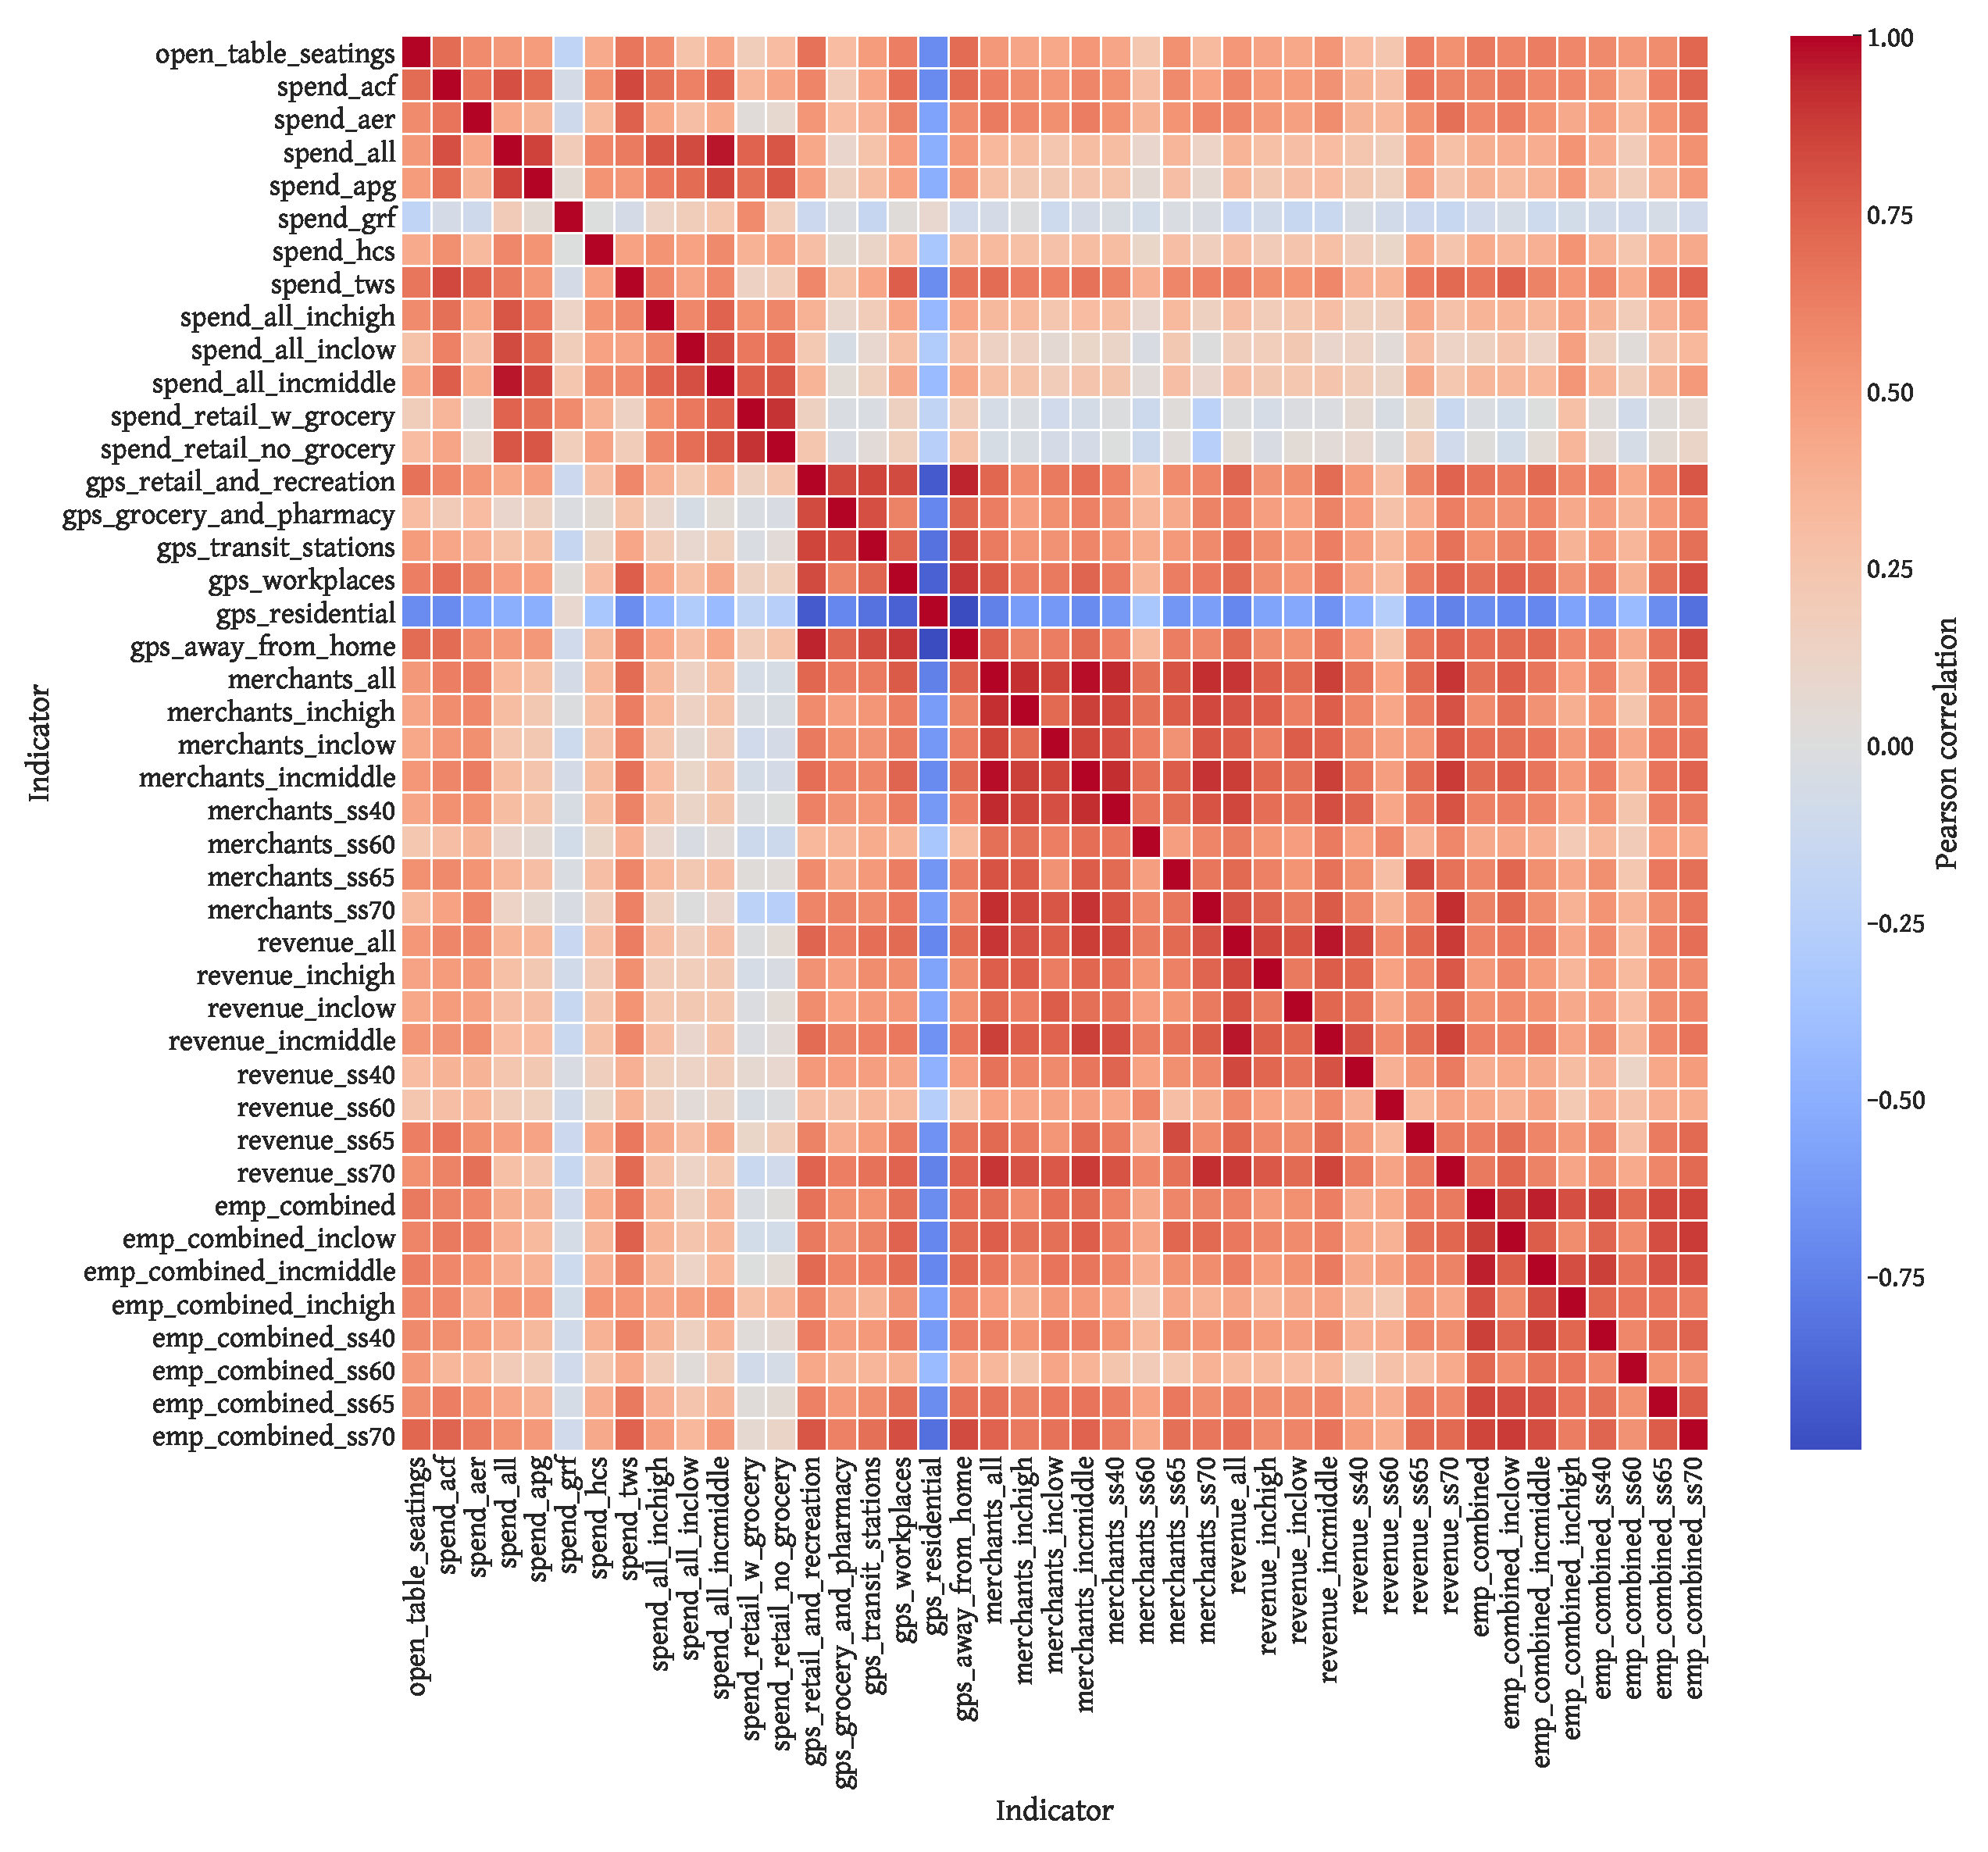
\includegraphics[width=0.9\textwidth]{corr_raw_indicators.eps}
    \caption{The pairwise correlation between each mobility indicator over the course of the pandemic across all US states. See the Opportunity Insights data dictionary on \href{https://github.com/OpportunityInsights/EconomicTracker/blob/main/docs/oi_tracker_data_dictionary.md}{GitHub} for a full description of each indicator.} % \ExternalLink was giving me TeX errors here...
    \label{fig:corr_raw_indicators}
\end{figure}

\begin{figure}
    \centering
    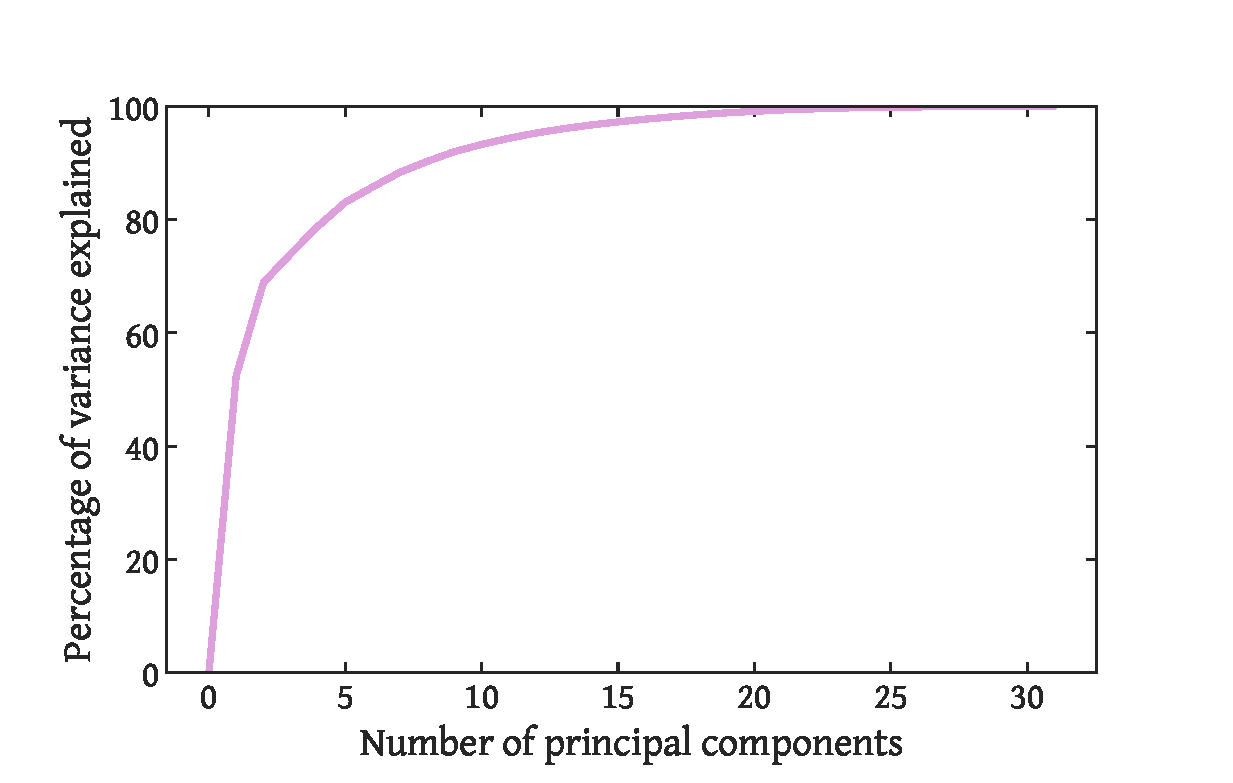
\includegraphics[width=0.6\textwidth]{cumulative_variance.eps}
    \caption{The cumulative percentage of variance explained by PCA when applied to the ensemble of social mobility data sources (see Section~\ref{sssec:extdata}).}
    \label{fig:cumulative_variance}
\end{figure}

\begin{figure}
    \centering
    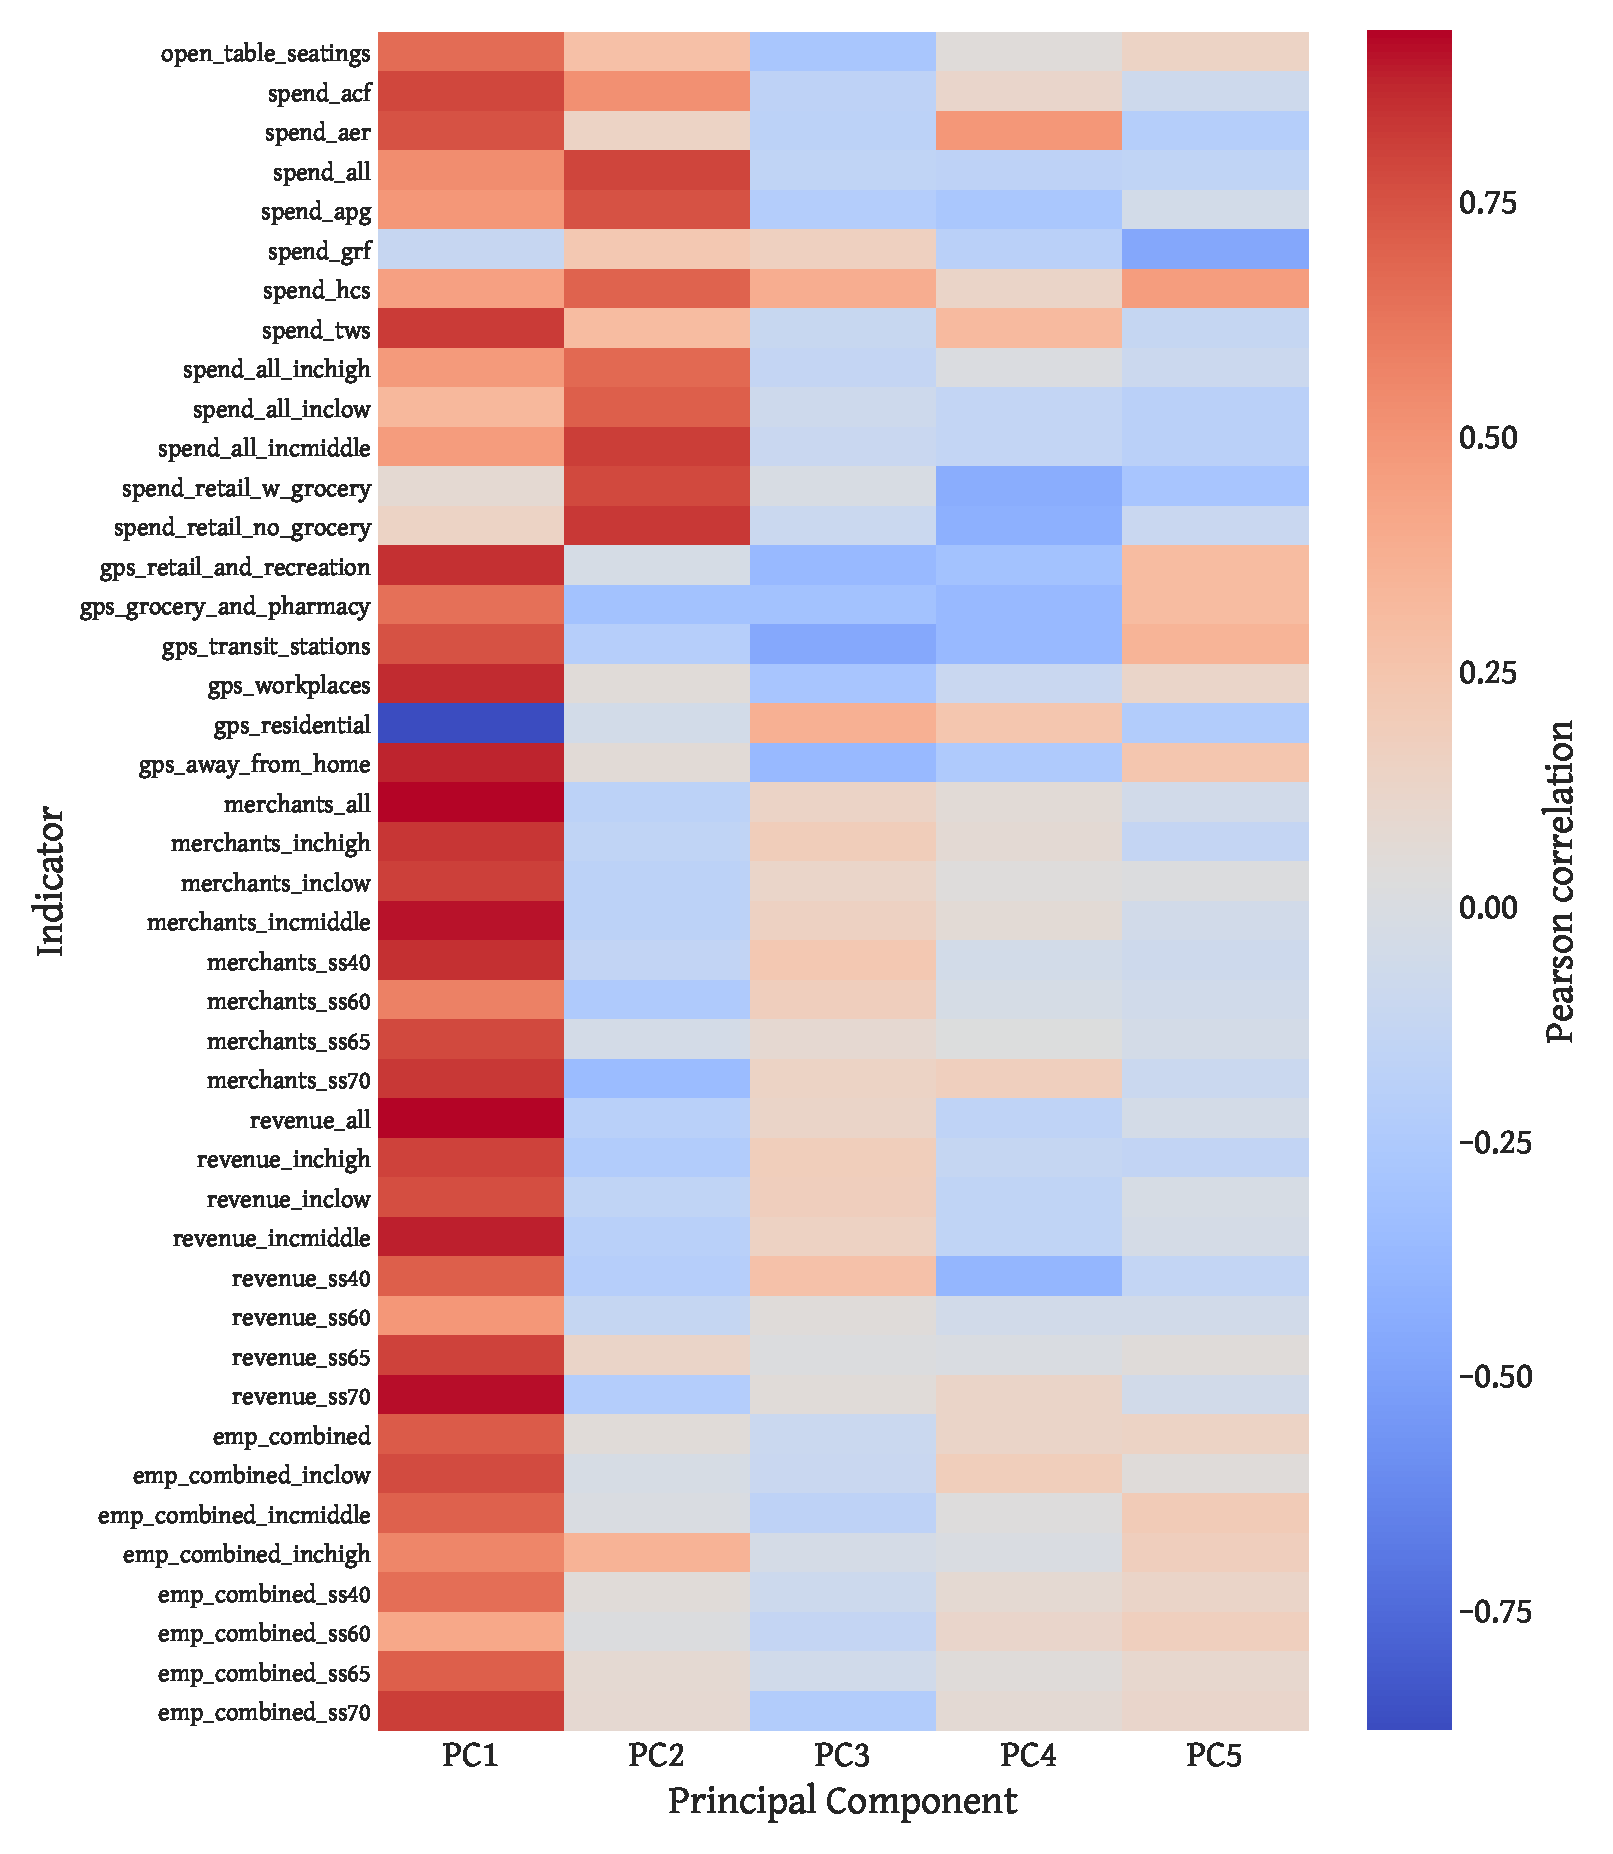
\includegraphics[width=0.9\textwidth]{corr_indicators_pca.eps}
    \caption{The correlation between each mobility indicator and projections along each of the first five principal components over the course of the pandemic across all US states. See the Opportunity Insights data dictionary on \href{https://github.com/OpportunityInsights/EconomicTracker/blob/main/docs/oi_tracker_data_dictionary.md}{GitHub} for a full description of each indicator.} % \ExternalLink was giving me TeX errors here...
    \label{fig:corr_indicators_pca}
\end{figure}

\begin{figure}
    \centering
    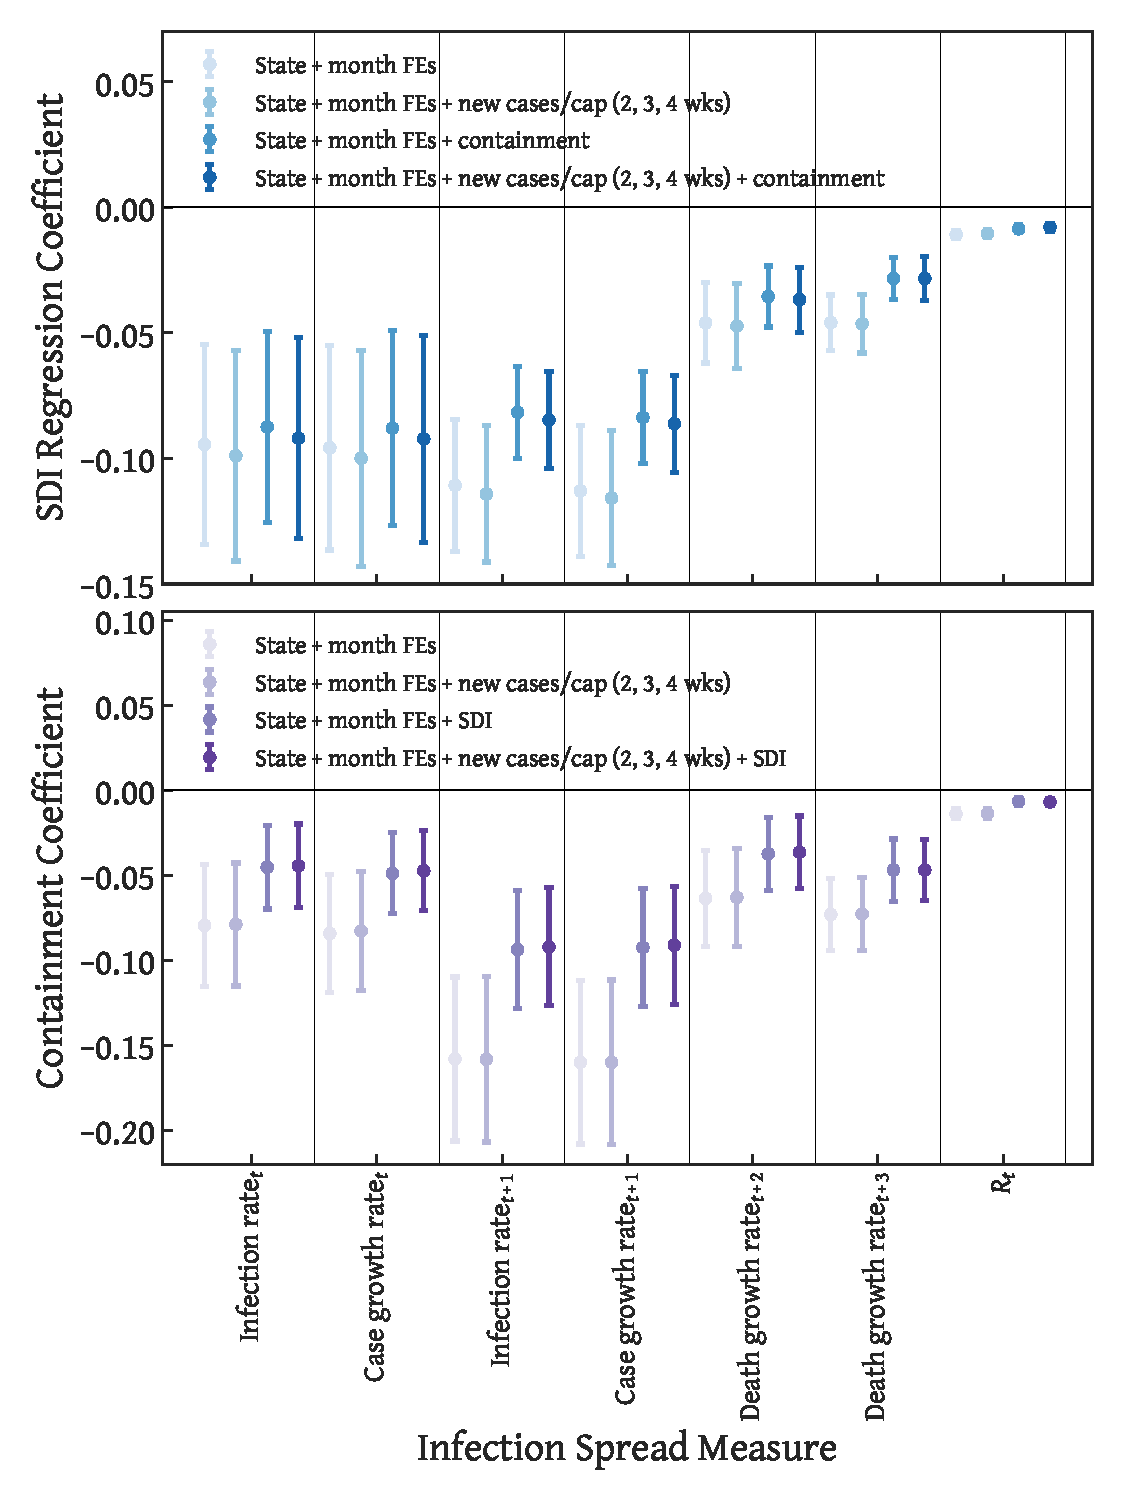
\includegraphics[width=0.8\textwidth]{sdi_containment_coefficients.eps}
    \caption{The regression coefficient (and corresponding 95\% confidence interval) for ({\it top}) the SDI and ({\it bottom}) the Containment Index in several regression models (described by the legend entries) used to predict different measures of spread.}
    \label{fig:sdi_containment_coefficients}
\end{figure}

\end{document}